\documentclass[12pt,a4paper]{report}

% ============================================================================
% PACKAGES & SETUP
% ============================================================================
\usepackage[english]{babel}
\usepackage[margin=2.5cm]{geometry}
\usepackage{mathptmx}          % Times New Roman equivalent
\usepackage{setspace}
\usepackage{graphicx}
\usepackage{fancyhdr}
\usepackage{tcolorbox}
\usepackage{hyperref}
\usepackage{xcolor}
\usepackage{listings}
\usepackage{float}
\usepackage{array}
\usepackage{booktabs}
\usepackage{amsmath}
\usepackage{amssymb}
\usepackage{tikz}
\usetikzlibrary{patterns}
\usepackage{svg}
\usepackage{subcaption}
\usepackage{xspace}

% Line spacing
\setstretch{1.15}

% Paragraph indentation
\parindent=0.5cm

% Page number setup
\pagestyle{fancy}
\fancyhf{}
\rfoot{\thepage/\pageref{LastPage}}
\renewcommand{\headrulewidth}{0pt}
\renewcommand{\footrulewidth}{0.4pt}

% Hyperref colors
\hypersetup{colorlinks=true, linkcolor=black, urlcolor=blue}

% Chapter formatting
\usepackage{titlesec}
\titleformat{\chapter}[display]
  {\normalfont\bfseries\fontsize{18}{20}\selectfont}
  {Chapter \thechapter}{0.5cm}{}
\titleformat{\section}
  {\normalfont\bfseries\fontsize{14}{16}\selectfont}
  {\thesection}{0.5cm}{}
\titleformat{\subsection}
  {\normalfont\bfseries\fontsize{12}{14}\selectfont}
  {\thesubsection}{0.5cm}{}

% Last page reference
\usepackage{lastpage}
\usepackage{pdfpages}

% ============================================================================
% DOCUMENT BEGIN
% ============================================================================
\begin{document}

% ============================================================================
% COVER PAGE
% ============================================================================
\includepdf[pages=-]{"Report/Page Garde Rapport Stage(Ang).pdf"}


% ============================================================================
% ACKNOWLEDGEMENTS
% ============================================================================
\chapter*{Acknowledgements}
\addcontentsline{toc}{chapter}{Acknowledgements}

I would like to express my sincere gratitude to all those who contributed to the success of this internship and the development of the Monetique Eye platform.

First and foremost, I thank my corporate supervisor, \textbf{Ahmed Ferchichi}, for his invaluable guidance, technical insights, and encouragement throughout the project. His feedback shaped the architecture and helped navigate complex decisions with clarity and pragmatism. Working alongside his team provided me with real-world exposure to enterprise systems and DevOps practices.

I am equally grateful to my academic supervisor, \textbf{Syrine Karoui}, for her thoughtful mentoring, constructive reviews, and support in translating technical work into a coherent academic narrative. Her guidance ensured that this project remained aligned with both practical and pedagogical objectives.

I also thank the broader Monetique team for fostering a collaborative and learning-oriented environment. Their willingness to discuss trade-offs, review designs, and share domain expertise accelerated my growth as a software engineer.

Finally, I acknowledge the open-source communities whose tools—Spring Boot, React, Prometheus, Elasticsearch, and many others—form the foundation of this platform. Their contributions to the software ecosystem made this ambitious project feasible within a six-month timeline.

This internship has been transformative. I leave with not only technical knowledge but also a deeper appreciation for thoughtful system design, cross-functional collaboration, and the importance of observability in modern infrastructure.

\newpage

% ============================================================================
% TABLE OF CONTENTS
% ============================================================================
\tableofcontents
\newpage

% ============================================================================
% GENERAL INTRODUCTION
% ============================================================================
\chapter*{General Introduction}
\addcontentsline{toc}{chapter}{General Introduction}

\section*{Context and Motivation}

Modern enterprise infrastructure has become increasingly complex. Organizations manage multiple environments (production, staging, development), distributed microservices, containers, virtual machines, and cloud resources—often spanning geographic regions and regulatory boundaries. In the financial services and payments sector (the \textit{monetique} domain), this complexity is compounded by stringent reliability requirements: any infrastructure failure directly impacts revenue, customer trust, and regulatory compliance.

Traditional infrastructure monitoring approaches suffer from significant limitations:

\begin{itemize}
  \item \textbf{Tool Fragmentation}: Separate platforms for metrics (Prometheus), logs (ELK stack), alerts (Alertmanager), and incidents create silos of information that operators must manually correlate.
  \item \textbf{Manual Provisioning}: Adding a new node for monitoring requires deep DevOps expertise—SSH key management, Ansible inventories, Prometheus targets, and logging agent configuration are often error-prone and time-consuming.
  \item \textbf{Lack of Intelligence}: Operators spend hours correlating logs, metrics, and alerts to understand root causes. AI-driven analysis is rare in traditional stacks.
  \item \textbf{Access Control Challenges}: Most monitoring platforms offer only coarse-grained RBAC, making it difficult to enforce environment-level data isolation in multi-tenant scenarios.
  \item \textbf{Deployment Tracking Gap}: CI/CD systems operate independently from observability, leaving operators without visibility into what was deployed and when.
\end{itemize}

\section*{Problem Statement}

This internship addresses a critical need: \textbf{How can enterprise IT teams unify fragmented observability tooling, automate infrastructure provisioning, and leverage AI to accelerate incident diagnosis—all within a single, secure, user-friendly platform?}

Specifically, we aimed to build a system that:

\begin{enumerate}
  \item Consolidates metrics, logs, alerts, and incident management into one intuitive interface
  \item Automates the deployment of monitoring agents on new infrastructure nodes
  \item Integrates AI (large language models) for automated log analysis and operational summarization
  \item Provides fine-grained role-based access control scoped by environment
  \item Integrates with existing GitOps workflows (Ansible, Jenkins) to avoid rip-and-replace
\end{enumerate}

\section*{Project Objectives}

The \textbf{Monetique Eye} project was structured to deliver an enterprise-grade observability platform through multiple sequential phases, each building upon the previous:

\begin{description}
  \item[Phase 1: Backend Foundation \& Security] Establish a secure, scalable data layer with JWT authentication, RBAC, and a minimal 10-entity data model.
  \item[Phase 2: Core UI \& Dashboarding] Build a React-based frontend with environment management, real-time monitoring dashboards, and an interactive topology visualization.
  \item[Phase 3: Advanced Observability Features] Implement log aggregation, real-time log search, and the AI-powered « Root Cause Intelligence » engine.
  \item[Phase 4: Operational Intelligence] Create executive dashboards with AI-generated summaries, stability scoring, and operational signal detection.
  \item[Phase 5: CI/CD Integration \& Hardening] Integrate Jenkins pipelines, implement automated deployment tracking, and harden security.
\end{description}

\section*{Chapter Overview}

This report documents the complete internship experience and the development of Monetique Eye:

\begin{itemize}
  \item \textbf{Chapter 1} presents the company context, the specific observability problem, and the initial requirements.
  \item \textbf{Chapter 2} explains the proposed architectural and technical approach, assuming a non-specialist reader.
  \item \textbf{Chapter 3} details the work realized across all five phases, including the planning, implementation challenges, and key design decisions. Diagrams and architecture visualizations are included throughout.
  \item The \textbf{Conclusion} synthesizes lessons learned, reflects on technical contributions, and suggests future research directions.
\end{itemize}

This report avoids raw code listings in the main text; technical implementation details and code snippets are deferred to the appendices. The focus is on \textbf{why} design choices were made and \textbf{how} they address the original problem.

\newpage

% ============================================================================
% CHAPTER 1: COMPANY & CONTEXT
% ============================================================================
\chapter{Company \& Context}

\section{Company Overview}

Monetique is a leading enterprise software company specializing in digital payment solutions and infrastructure services for the financial sector. The company operates globally, managing critical payment processing systems, transaction platforms, and enterprise middleware solutions for hundreds of financial institutions, retailers, and payment processors.

The organization's infrastructure and platform division—where this internship was conducted—focuses on building resilient, scalable systems for their clients. The teams manage complex multi-cluster deployments, monitor mission-critical payment gateways, and ensure continuous service availability. Given the financial nature of the business, any infrastructure downtime directly impacts transactions and customer satisfaction.

\section{The Department: Infrastructure \& Observability}

The internship was embedded within the \textbf{Infrastructure and Observability} department, a team of approximately 20 engineers responsible for:

\begin{itemize}
  \item Designing and operating the company's private cloud platform
  \item Managing multi-environment deployments (production, staging, development)
  \item Implementing monitoring and alerting infrastructure
  \item Providing operational support (24/7 on-call rotations for critical systems)
  \item Building internal tools for DevOps automation
\end{itemize}

The department already operated a fragmented observability stack: Prometheus for metrics, Elasticsearch for logs, Grafana for visualization, and Ansible for infrastructure automation. However, no unified platform existed to tie these tools together—operators still performed manual correlation and root cause analysis.

\section{Initial Problem Statement}

At the start of the internship, the team articulated a specific pain point:

\begin{quote}
  « When an incident occurs, our operators face a 45-minute investigation window: they manually SSH into servers, grep logs, run ad-hoc Prometheus queries, and correlate events across multiple dashboards. By the time we've diagnosed the root cause, customer impact has already accumulated. We need a unified observability platform with intelligent diagnostics to cut incident resolution time in half. »
\end{quote}

Additionally, provisioning new monitoring infrastructure was cumbersome: adding a client node for monitoring required a DevOps engineer to manually configure SSH keys, Ansible inventories, Prometheus targets, and logging agents—a process that typically took 2–4 hours per node.

\section{Scope and Feasibility}

Given a six-month internship window, the team and I agreed on the following scope:

\begin{itemize}
  \item Build a full-stack application (backend API + React UI + MySQL database)
  \item Automate infrastructure provisioning through a one-click deployment interface
  \item Integrate the existing Prometheus, Elasticsearch, and Ansible stack (no replacement)
  \item Implement RBAC and multi-environment isolation
  \item Add AI-powered log analysis using a large language model API
  \item Provide enough flexibility for future enhancements (phases 6 and beyond)
\end{itemize}

Out of scope (deferred to future phases):
\begin{itemize}
  \item Kubernetes-native deployment (only Docker + VMs in scope)
  \item Custom machine learning model training
  \item Advanced predictive analytics
\end{itemize}

\section{Key Stakeholders}

\begin{center}
\begin{tabular}{|l|l|p{5cm}|}
  \hline
  \textbf{Stakeholder} & \textbf{Role} & \textbf{Key Concerns} \\
  \hline
  CTO / VP Engineering & Project Sponsor & ROI, timeline, technical feasibility \\
  \hline
  DevOps Team Lead & Product Owner & Ease of use, integration with existing tools \\
  \hline
  SRE Team & Primary Users & Speed of incident diagnosis, alert quality \\
  \hline
  Backend Team & Integration Partner & API design, data security \\
  \hline
  Security Officer & Compliance & Authentication, RBAC, audit logging \\
  \hline
\end{tabular}
\end{center}

\section{Chapter 1 Summary}

Monetique operates in a high-stakes domain where infrastructure reliability directly translates to business outcomes. The existing observability tooling, while capable, requires significant manual effort to operate. This project aimed to unify and simplify the operational experience through a modern, integrated platform—one that automates routine tasks and accelerates incident diagnosis through intelligent analysis. The clear problem statement, defined scope, and engaged stakeholders provided a solid foundation for execution.

\newpage

% ============================================================================
% CHAPTER 2: PROPOSED WORK DESCRIPTION
% ============================================================================
\chapter{Proposed Work Description}

\section{High-Level Solution Architecture}

The Monetique Eye platform is designed around a « push-button infrastructure » model: a user clicks a single button in the UI, and the backend orchestrates all necessary provisioning, configuration, and registration steps without requiring manual intervention.

Figure \ref{fig:context} illustrates the overall system context:

\begin{figure}[H]
  \centering
  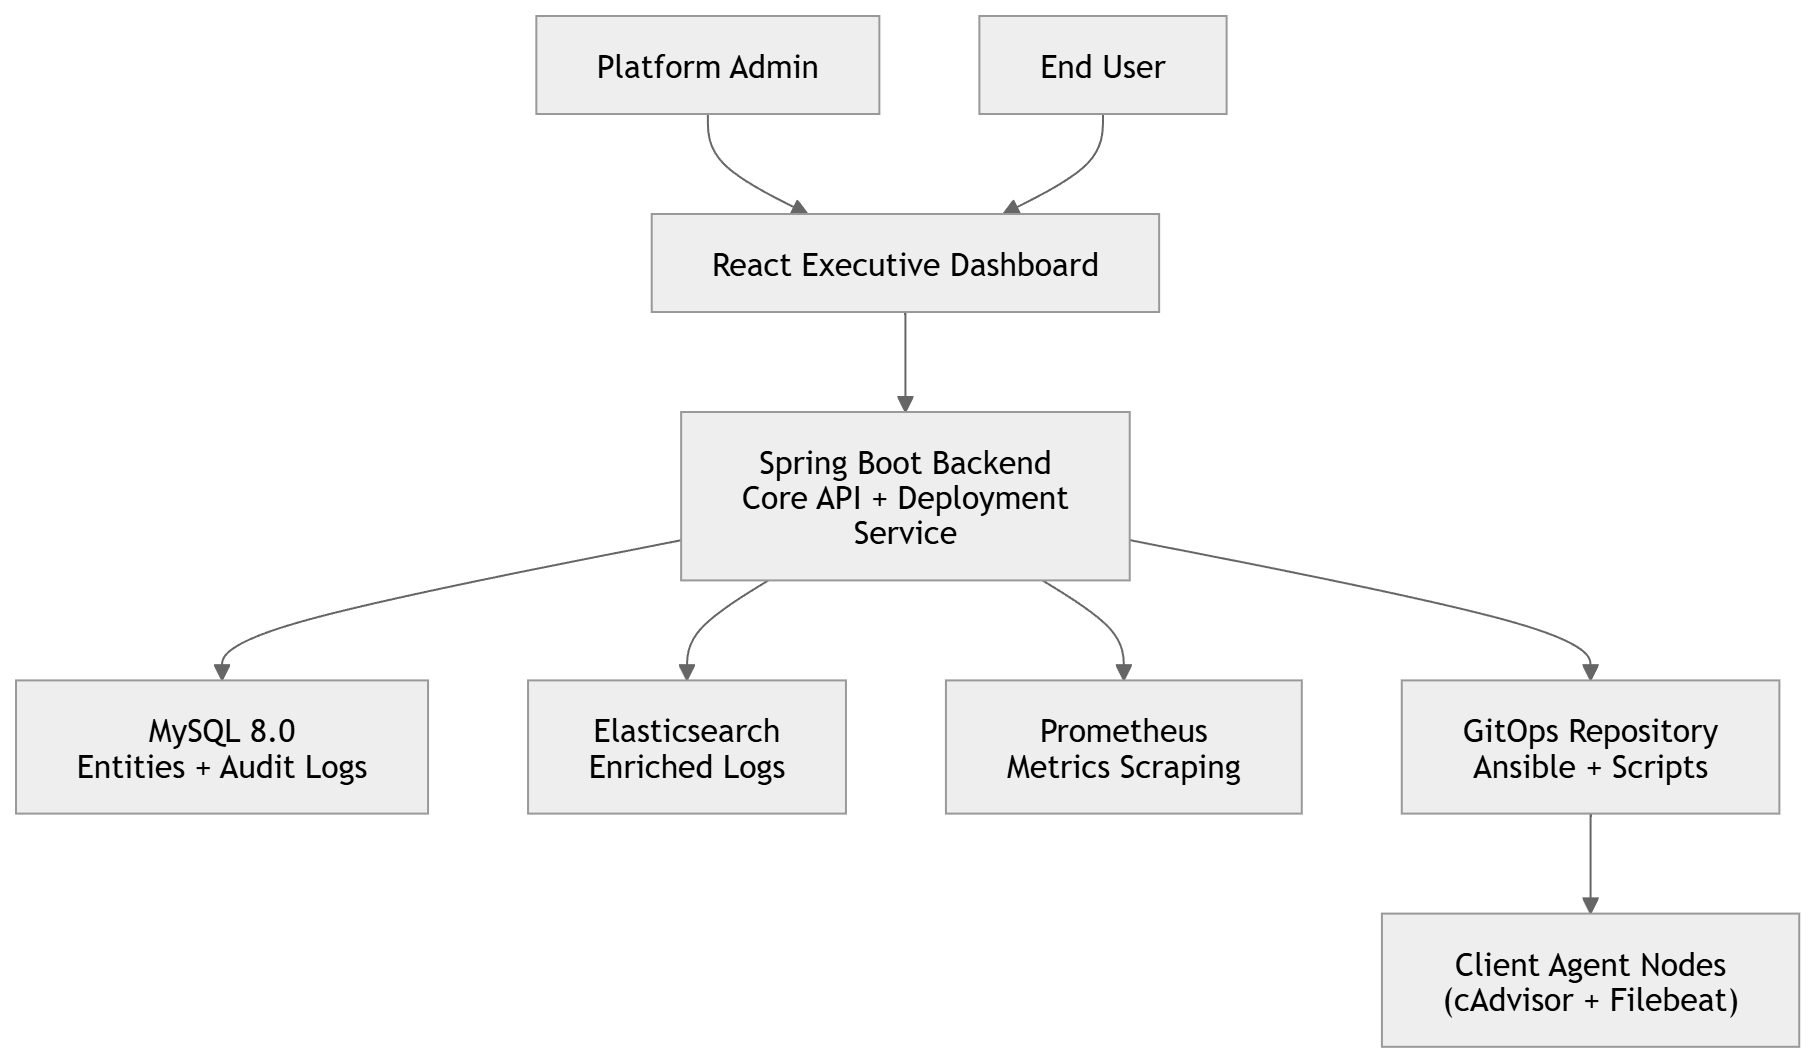
\includegraphics[width=0.85\textwidth]{documentation/diagram/Clean_C4Context_Diagram.png}
  \caption{C4 Context Diagram: Monetique Eye System Boundaries}
  \label{fig:context}
\end{figure}

The system consists of four major layers:

\begin{description}
  \item[Data Ingestion Layer] Remote nodes deploy monitoring agents (Node Exporter, cAdvisor, Filebeat) that emit metrics to Prometheus and logs to the central ELK stack.
  \item[Backend Orchestration Layer] A Spring Boot API orchestrates Ansible playbooks, manages environments and applications, and correlates observability data.
  \item[Data Processing Layer] Elasticsearch and Prometheus perform aggregations; the backend queries these systems to compute analytics and root cause signals.
  \item[Presentation Layer] A React-based dashboard provides operators with consolidated visibility and one-click control.
\end{description}

\section{Technical Problem: Why Build This?}

\subsection{The Fragmentation Challenge}

Traditional infrastructure monitoring suffers from what we call « observability fragmentation »: data lives in silos, and operators must manually jump between tools. Consider a typical incident:

\begin{enumerate}
  \item An alert fires from Alertmanager: « CPU spike on node-42 »
  \item Operator logs into Grafana to see the CPU metric
  \item Operator logs into Kibana (ELK) to search for application errors during the spike
  \item Operator SSH's into the node to check running processes
  \item Operator cross-references deployment logs with the timeline
  \item Finally, operator identifies the root cause: a slow database query introduced in a recent deploy
\end{enumerate}

This process is \textbf{manual}, \textbf{slow}, and \textbf{error-prone}. Monetique Eye automates this correlation using structured data integration and intelligent analysis.

\subsection{The Provisioning Challenge}

Onboarding a new monitored node traditionally requires:
\begin{enumerate}
  \item Generate and distribute SSH keys
  \item Manually edit Ansible inventory files
  \item Configure Prometheus targets and scrape rules
  \item Deploy logging agents and configure pipelines
  \item Verify connectivity and metric flow
\end{enumerate}

This takes hours. Monetique Eye encapsulates this workflow into a single backend function, triggered by a UI button click.

\subsection{The Access Control Challenge}

Existing monitoring tools typically operate in « all-or-nothing » mode: either a user sees all environments, or they see nothing. Enterprise clients require \textbf{environment-level} isolation—a « Staging » team member should not see « Production » data. The platform must enforce this at the data layer.

\section{Proposed Solution: The Five-Phase Approach}

To deliver a robust, production-grade platform within the six-month internship, we structured development into five sequential phases:

\subsection{Phase 1: Backend Foundation \& Security}

\textbf{Objectives:}
\begin{itemize}
  \item Design and implement a minimal, clean data model (10 core entities)
  \item Establish stateless JWT-based authentication
  \item Implement role-based access control (RBAC) at the entity level
  \item Create the foundational APIs for environment and application management
\end{itemize}

\textbf{Key Technologies:}
\begin{itemize}
  \item Spring Boot 3.3 with Spring Security
  \item Hibernate/JPA with MySQL 8.0
  \item JSON Web Tokens (JWT) with jjwt library
  \item BCrypt password hashing
\end{itemize}

\subsection{Phase 2: Core UI \& Dashboarding}

\textbf{Objectives:}
\begin{itemize}
  \item Build a modern, responsive React UI with Tailwind CSS
  \item Implement environment management interface
  \item Create real-time monitoring dashboards displaying Prometheus metrics
  \item Implement an interactive topology graph using React Flow
\end{itemize}

\textbf{Key Technologies:}
\begin{itemize}
  \item React 18 with Vite for fast development and builds
  \item Tailwind CSS for responsive, utility-first styling
  \item React Flow for interactive topology visualization
  \item Axios for API communication
\end{itemize}

\subsection{Phase 3: Advanced Observability Features}

\textbf{Objectives:}
\begin{itemize}
  \item Implement one-click agent deployment (backend → Ansible → remote nodes)
  \item Integrate Elasticsearch for centralized log aggregation and search
  \item Build a « Root Cause Intelligence » engine that correlates logs and metrics
  \item Create structured SRE signal extraction from logs
\end{itemize}

\textbf{Key Technologies:}
\begin{itemize}
  \item Elasticsearch Query DSL for aggregated log analysis
  \item Prometheus query language (PromQL) for metric correlation
  \item Ansible for infrastructure automation
  \item Docker and SSH for remote execution
\end{itemize}

\subsection{Phase 4: Operational Intelligence}

\textbf{Objectives:}
\begin{itemize}
  \item Integrate a large language model (Groq Llama 3.3) for AI-powered diagnostics
  \item Create an « Operational Intelligence » dashboard with stability scoring
  \item Implement log drift analysis and recurring issue detection
  \item Build an AI chat assistant with infrastructure context
\end{itemize}

\textbf{Key Technologies:}
\begin{itemize}
  \item Groq API for fast LLM inference
  \item Z-score statistical analysis for stability scoring
  \item Embedding-based semantic log similarity
\end{itemize}

\subsection{Phase 5: CI/CD Integration \& Hardening}

\textbf{Objectives:}
\begin{itemize}
  \item Integrate Jenkins pipelines for application deployment
  \item Implement deployment event recording and tracking
  \item Enhance security with additional audit logging and validation
  \item Optimize performance and reliability for production
\end{itemize}

\textbf{Key Technologies:}
\begin{itemize}
  \item Jenkins REST API integration
  \item Docker Registry for container image management
  \item Extended audit logging
\end{itemize}

\section{Data Model: Environment-First Design}

At the core of Monetique Eye is a hierarchical, environment-scoped data model:

\begin{figure}[H]
  \centering
  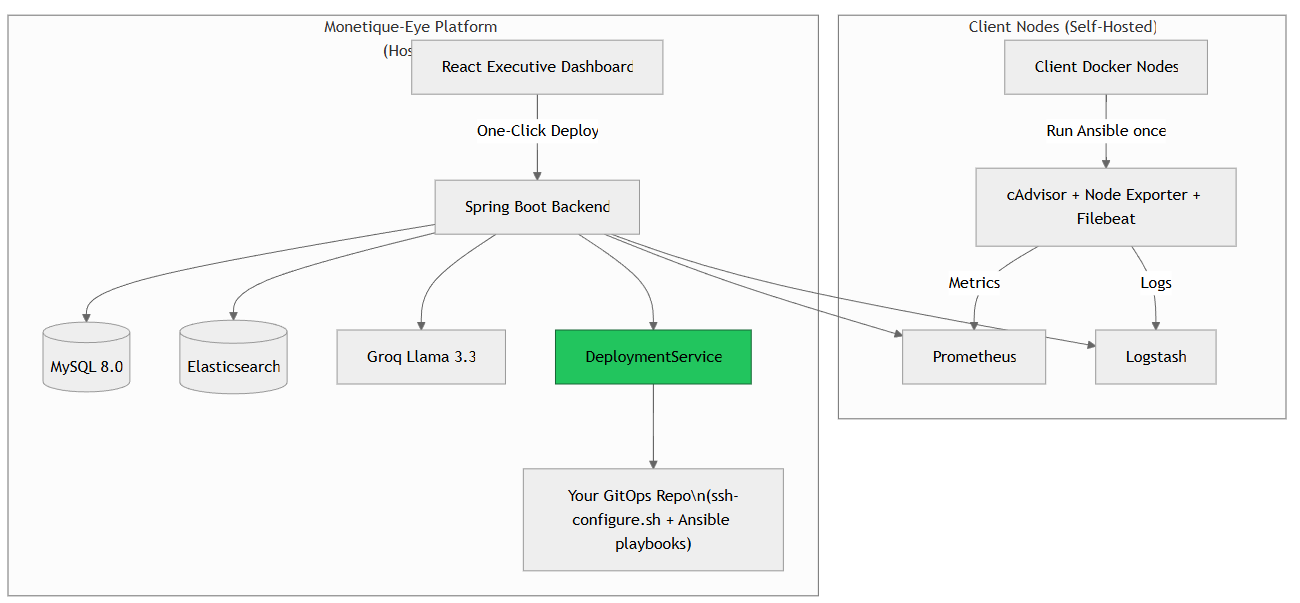
\includegraphics[width=0.8\textwidth]{documentation/diagram/GLOBAL_ARCHITECTURE_DIAGRAM.png}
  \caption{Global Architecture and Data Flow}
  \label{fig:architecture}
\end{figure}

All data—applications, nodes, metrics, logs, alerts, incidents—are scoped to an \textbf{Environment}. This ensures:
\begin{itemize}
  \item \textbf{Multi-tenancy}: Different clients or business units can operate independently
  \item \textbf{RBAC Enforcement}: A user granted « USER » role on « Staging » cannot access « Production »
  \item \textbf{Logical Isolation}: Prometheus, Elasticsearch, and alert rules operate independently per environment
\end{itemize}

\section{Key Design Principles}

\begin{description}
  \item[Minimal Data Model] Only 10 core entities to reduce cognitive load and maintenance burden
  \item[No Vendor Lock-in] Reuses existing GitOps, Ansible, Prometheus, and ELK tooling
  \item[Zero-Config Discovery] Monitoring agents auto-register; operators see live data within seconds
  \item[Stateless APIs] No session state; all requests are validated via JWT
  \item[Asynchronous Orchestration] Long-running tasks (deployments) don't block the UI
  \item[Audit Everything] All actions are logged for compliance and troubleshooting
\end{description}

\section{Chapter 2 Summary}

Monetique Eye solves real operational pain points through architectural innovations: consolidating fragmented tooling, automating provisioning, and integrating intelligent analysis. The five-phase approach balances ambition with feasibility, delivering a production-grade platform in six months. The environment-first data model and stateless architecture provide a solid foundation for multi-tenant enterprise use.

\newpage

% ============================================================================
% CHAPTER 3: REALIZED WORK
% ============================================================================
\chapter{Realized Work}

\section{Internship Planning \& Timeline}

The internship was structured as a six-month, full-time engagement spanning January through June 2026. The phases were designed to deliver functionality incrementally, with clear checkpoints for validation and feedback.

\subsection{Gantt Chart}

The figure below illustrates the project timeline, key phases, and deliverables:

\begin{figure}[H]
  \centering
  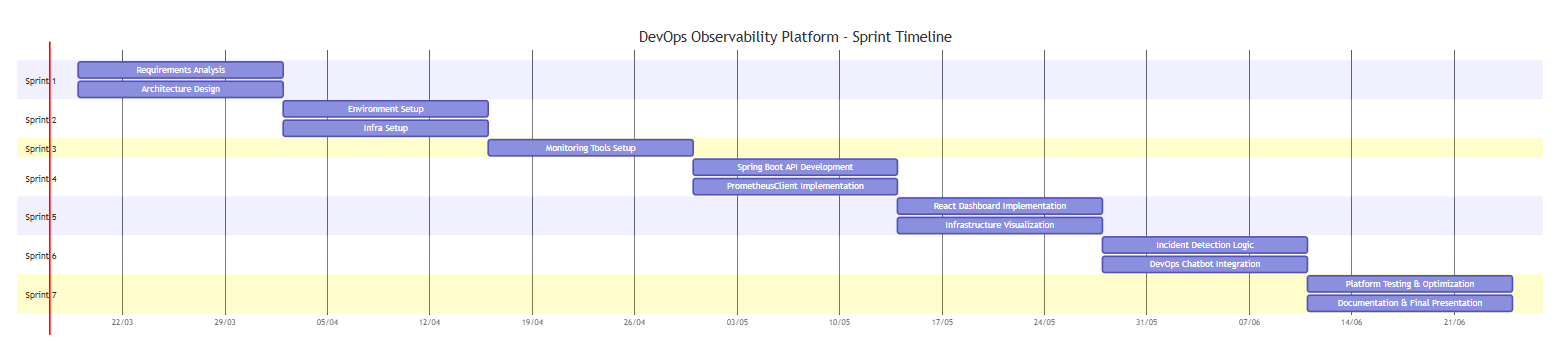
\includegraphics[width=\textwidth]{documentation/diagram/Diagram_de_gantt.png}
  \caption{Internship Gantt Chart: Six-Month Project Timeline}
  \label{fig:gantt}
\end{figure}

\textbf{Key Milestones:}

\begin{itemize}
  \item \textbf{End of January (Phase 1):} Secure backend with JWT authentication, RBAC, and database schema
  \item \textbf{End of February (Phase 2):} Functional React UI with environment management and dashboarding
  \item \textbf{End of March (Phase 3):} One-click deployment, log aggregation, Root Cause Intelligence engine
  \item \textbf{End of April (Phase 4):} AI-powered operational intelligence dashboards
  \item \textbf{End of May (Phase 5):} CI/CD integration, security hardening, production readiness
  \item \textbf{June:} Performance optimization, documentation, and internal deployment
\end{itemize}

\section{Methodology: Agile with Kanban}

\subsection{Why Kanban?}
The project scope evolved continuously as new infrastructure requirements emerged. Kanban's visual task board and pull-based flow allowed priorities to be reprioritized at any time without disrupting delivery, making it a better fit than time-boxed Scrum sprints for a solo engineering context.

\subsection{Sprint Detail}
Although guided by Kanban, the work was naturally grouped into functional sprints or phases to ensure iterative delivery:
\begin{itemize}
    \item \textbf{Sprint 1:} Requirements analysis and functional scoping. System architecture design (layers, tech stack selection).
    \item \textbf{Sprint 2:} Docker Compose environment setup (14 containers). Infrastructure provisioning: network, volumes, secrets.
    \item \textbf{Sprint 3:} Prometheus, Grafana, ELK, Alertmanager full setup. Scrape jobs, alert rules, log pipeline configuration.
    \item \textbf{Sprint 4:} Spring Boot REST API (31 controllers, 25 entities). PrometheusClient + Alertmanager webhook integration.
    \item \textbf{Sprint 5:} React 19 SPA (21 pages, protected routes, Recharts). Infrastructure topology graph (React Flow).
    \item \textbf{Sprint 6:} Incident detection, alerting pipeline, ticket linking. AI Chatbot integration (Groq Llama 3.3, WebClient).
    \item \textbf{Sprint 7:} End-to-end testing, performance optimization. Documentation, final presentation preparation.
\end{itemize}

\section{Phase 1: Backend Foundation \& Security}

\subsection{Overview}

Phase 1 established the platform's data and security layer. The goal was to create a minimal, clean backend that could scale and remain maintainable.

\subsection{Data Model Design}

We designed exactly 10 core entities, organized by functional domain:

\begin{center}
\begin{tabular}{|l|l|p{4cm}|}
  \hline
  \textbf{Entity} & \textbf{Purpose} & \textbf{Key Fields} \\
  \hline
  \texttt{Environment} & Top-level container for all data & name, cluster, labels \\
  \hline
  \texttt{Application} & Deployed service in an environment & name, type, status \\
  \hline
  \texttt{User} & Platform user with roles & username, email, roles \\
  \hline
  \texttt{Ticket} & Incident tracking & title, status, priority \\
  \hline
  \texttt{DeploymentLog} & Audit trail for Ansible runs & timestamp, environment, status \\
  \hline
  \texttt{Incident} & Auto-detected system alerts & severity, description, timestamp \\
  \hline
  \texttt{LogAggregationWindow} & Stability metrics & environment, window, score \\
  \hline
  \texttt{RecurringPattern} & Detected log anomalies & name, frequency, pattern \\
  \hline
  \texttt{AiOperationalSummary} & AI-generated digests & content, timestamp, environment \\
  \hline
  \texttt{Conversation} & AI chat history & userId, messages, context \\
  \hline
\end{tabular}
\end{center}

This minimal model reduces complexity while covering all essential use cases. All entities are scoped to an \texttt{Environment}, enforcing multi-tenancy at the database schema level.

\subsection{Authentication \& Authorization}

We implemented a stateless JWT-based authentication system:

\begin{enumerate}
  \item Client sends credentials (username/password) to \texttt{/api/v1/auth/login}
  \item Server validates credentials against BCrypt-hashed passwords in the database
  \item Server issues a signed JWT token with embedded user ID, role, and environment scope
  \item Client includes the JWT in the \texttt{Authorization} header for subsequent requests
  \item Server validates the token signature and checks RBAC permissions on each request
\end{enumerate}

\textbf{Security Features:}
\begin{itemize}
  \item \textbf{BCrypt Hashing:} All user passwords are hashed with BCrypt (not reversible)
  \item \textbf{JWT Signing:} Tokens are signed with a 256-bit secret key, preventing tampering
  \item \textbf{Token Expiration:} Tokens expire after 24 hours (configurable)
  \item \textbf{Refresh Tokens:} A separate refresh token allows clients to obtain new access tokens without re-entering credentials
  \item \textbf{CORS Protection:} Cross-origin requests are validated and restricted to trusted domains
\end{itemize}

\subsection{RBAC Foundation}

We implemented two primary roles:

\begin{description}
  \item[ADMIN] Full platform access; can create/delete environments, deploy agents, manage users
  \item[USER] Read-only access to assigned environments; can view dashboards and create tickets
\end{description}

The backend enforces RBAC using Spring Security's \texttt{@PreAuthorize} annotations on controller methods. Each user entity stores an explicit list of environment IDs they have access to, enabling fine-grained isolation.

\subsection{REST API Endpoints (Phase 1)}

By the end of Phase 1, we established the foundational API structure:

\begin{center}
\begin{tabular}{|l|l|l|}
  \hline
  \textbf{Endpoint} & \textbf{Method} & \textbf{Description} \\
  \hline
  \texttt{/api/v1/auth/login} & POST & Authenticate and obtain JWT \\
  \hline
  \texttt{/api/v1/environments} & GET/POST & List/create environments \\
  \hline
  \texttt{/api/v1/applications} & GET/POST & List/create applications \\
  \hline
  \texttt{/api/v1/users} & GET/POST (ADMIN only) & User management \\
  \hline
  \texttt{/api/v1/tickets} & GET/POST & Ticket lifecycle \\
  \hline
\end{tabular}
\end{center}

\section{Phase 2: Core UI \& Dashboarding}

\subsection{Overview}

Phase 2 focused on building an intuitive, modern user interface using React, Vite, and Tailwind CSS. The goal was to provide operators with a consolidated view of their infrastructure and a simple interface to manage environments.

\subsection{Frontend Architecture}

The React application was organized into clear functional domains:

\begin{itemize}
  \item \textbf{Pages}: Seven core pages handling different workflows
  \item \textbf{Components}: Reusable UI components (cards, tables, modals)
  \item \textbf{Services}: API clients for communication with the backend
  \item \textbf{Context}: Global state management for user authentication and environment selection
  \item \textbf{Types}: TypeScript interfaces for type safety
\end{itemize}

\subsection{Key Pages Implemented}

\begin{description}
  \item[Dashboard Page] High-level overview of system health, active alerts, and key metrics
  \item[Environments Page] CRUD interface for environment management
  \item[Applications Page] Manage deployed applications and their monitoring status
  \item[Infrastructure Topology] Interactive graph visualization of clusters and nodes
  \item[Logs Page] Search and filter logs from Elasticsearch
  \item[Tickets Page] Incident tracking and collaboration interface
  \item[Chat Page] AI assistant interface (implemented in Phase 4)
\end{description}

\subsection{Real-Time Monitoring Dashboard}

The Dashboard page displays the « Golden Signals » for infrastructure health:

\begin{figure}[H]
  \centering
  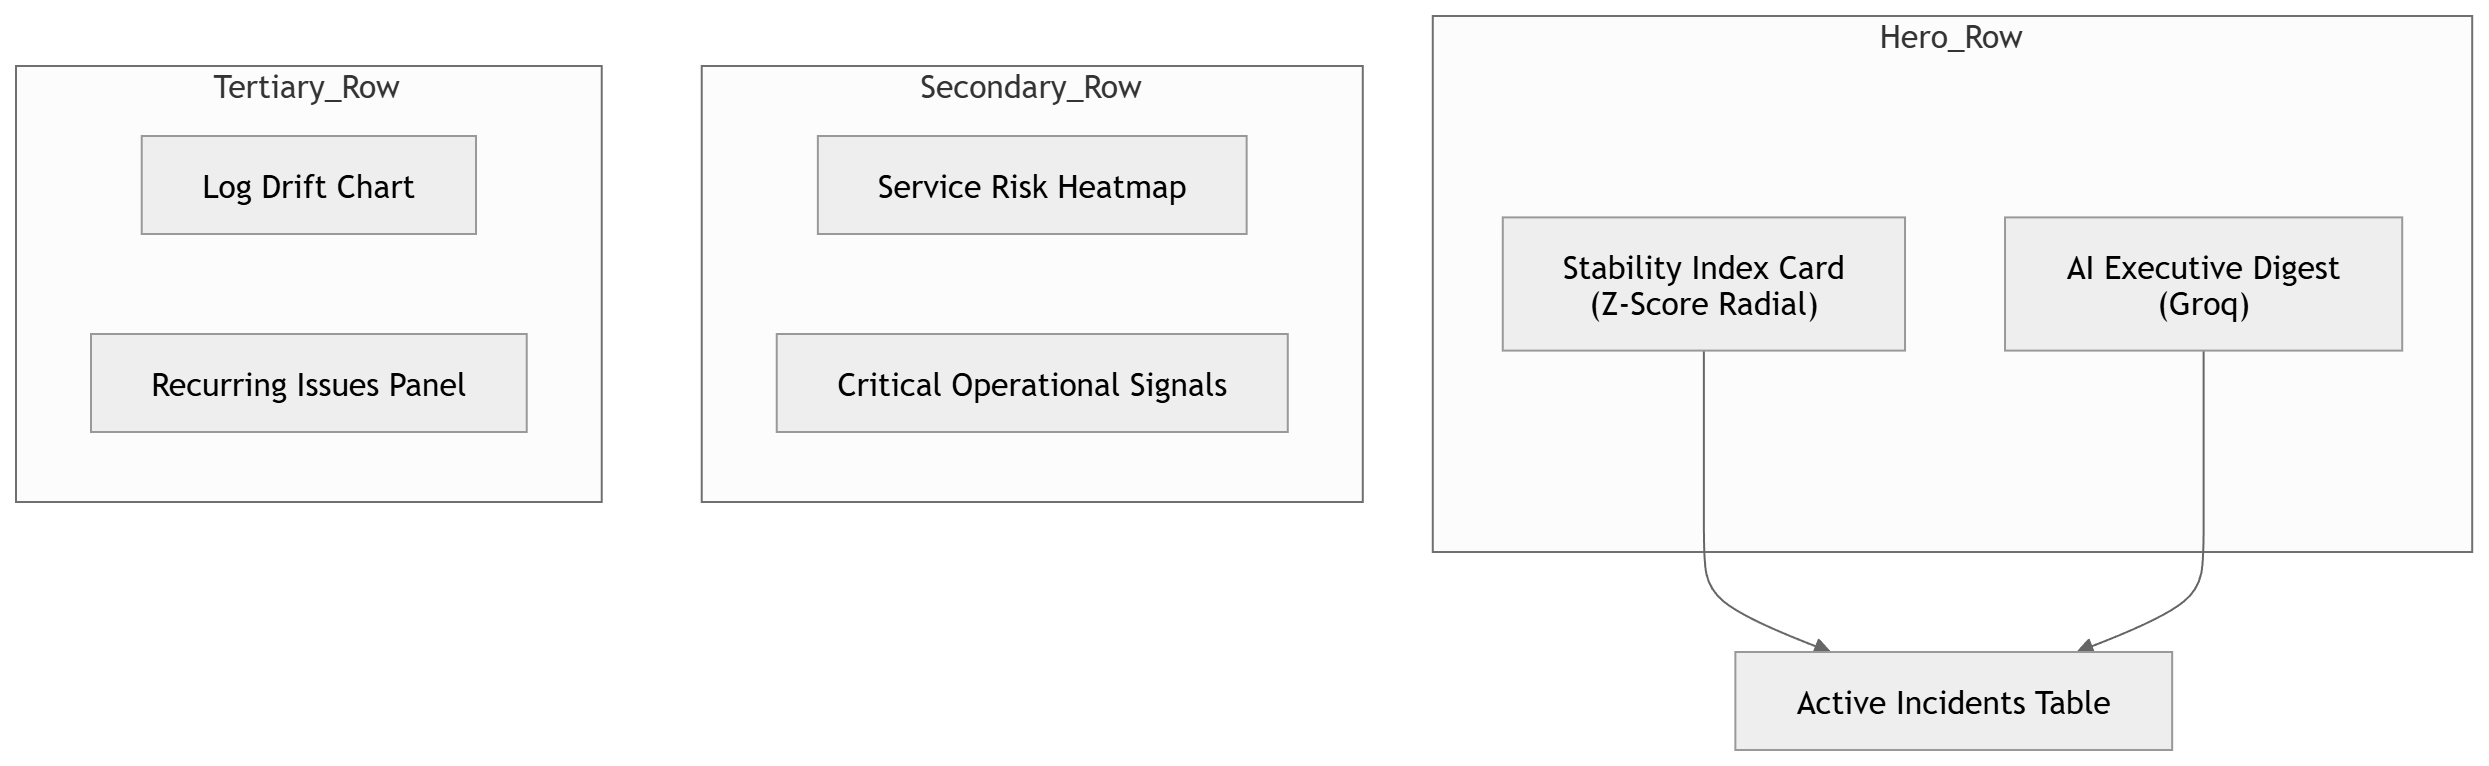
\includegraphics[width=0.75\textwidth]{documentation/diagram/Operational_Intelligence_Dashboard_Component_Layout_Diagram.png}
  \caption{Operational Intelligence Dashboard Layout}
  \label{fig:dashboard_layout}
\end{figure}

The dashboard fetches Prometheus metrics and displays:
\begin{itemize}
  \item \textbf{CPU Usage} - Container-level CPU consumption
  \item \textbf{Memory Usage} - Resident set size in MB
  \item \textbf{Network I/O} - Inbound/outbound throughput
  \item \textbf{Disk Usage} - Filesystem consumption
\end{itemize}

Data is refreshed every 30 seconds, providing near real-time visibility.

\subsection{Interactive Topology Visualization}

Using React Flow, we implemented an interactive graph showing cluster hierarchy:

\begin{figure}[H]
  \centering
  \includegraphics[width=0.75\textwidth]{"documentation/diagram/Infrastructure Visibility \& Topology Flow.png"}
  \caption{Infrastructure Visibility and Topology Flow Diagram}
  \label{fig:topology_flow}
\end{figure}

The topology dynamically renders:
\begin{itemize}
  \item Cluster nodes at the top level
  \item Environment nodes nested within clusters
  \item Application/service nodes within environments
  \item Live status indicators (green = healthy, red = degraded)
\end{itemize}

Users can click on nodes to drill down, zoom in/out, and inspect detailed metrics.

\section{Phase 3: Advanced Observability Features}

\subsection{Overview}

Phase 3 introduced the platform's core observability innovation: one-click agent deployment and intelligent log correlation.

\subsection{One-Click Deployment}

\textbf{The Problem:} Traditionally, provisioning monitoring on a new node requires:
\begin{enumerate}
  \item SSH key generation and distribution
  \item Manual Ansible inventory updates
  \item Prometheus target configuration
  \item Logging agent deployment
  \item Verification of data flow
\end{enumerate}

\textbf{The Solution:} We created an automated deployment orchestration layer:

\begin{figure}[H]
  \centering
  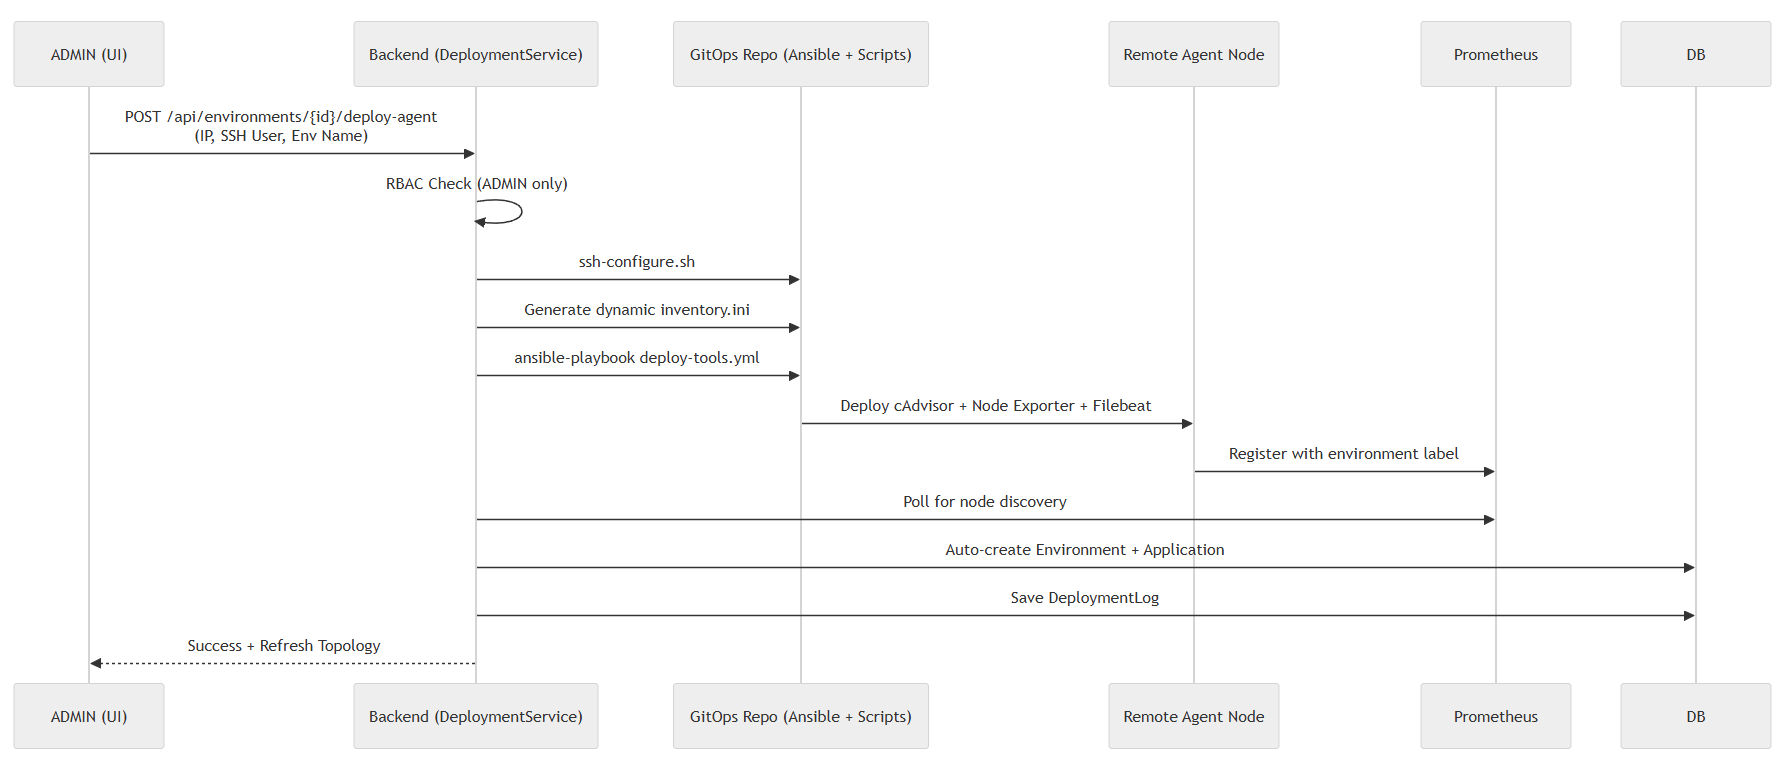
\includegraphics[width=0.8\textwidth]{documentation/diagram/Sequences_Environment_Management.png}
  \caption{Automated Deployment Sequence Diagram}
  \label{fig:deployment_sequence}
\end{figure}

The workflow:
\begin{enumerate}
  \item Admin clicks « Deploy » in the UI
  \item Backend validates permissions (ADMIN check)
  \item Backend executes \texttt{ssh-configure.sh} to establish connectivity
  \item Backend generates a dynamic Ansible inventory based on the environment definition
  \item Backend executes \texttt{deploy-tools.yml} playbook:
    \begin{itemize}
      \item Installs Node Exporter for metrics
      \item Installs cAdvisor for container metrics
      \item Installs Filebeat for log aggregation
      \item Configures all tools to point to the central observability stack
    \end{itemize}
  \item Deployment status is recorded in the database
  \item Backend polls Prometheus to confirm metrics are flowing
  \item Frontend shows « Deployment Successful » and live data
\end{enumerate}

The entire process takes 2–3 minutes (vs. 2–4 hours manual setup), and operators never touch SSH or Ansible directly.

\subsection{Elasticsearch Integration}

Phase 3 integrated centralized log aggregation:

\begin{itemize}
  \item \textbf{Filebeat} ships logs from application containers to the ELK stack
  \item \textbf{Logstash} normalizes and parses logs from multiple sources
  \item \textbf{Elasticsearch} stores and indexes logs for fast, full-text search
  \item \textbf{Backend API} provides a query interface to retrieve logs from the UI
\end{itemize}

The Log Search page allows operators to filter logs by:
\begin{itemize}
  \item Environment
  \item Application name
  \item Severity level
  \item Time range
  \item Full-text search terms
\end{itemize}

\subsection{Root Cause Intelligence Engine}

The « Root Cause Intelligence Engine » is the intellectual core of Phase 3. It correlates multiple data sources to identify the likely root cause of an incident.

\textbf{Signal Extraction Strategy:}

The engine extracts structured « SRE signals » from logs, representing common failure modes:

\begin{center}
\begin{tabular}{|l|l|}
  \hline
  \textbf{Signal} & \textbf{Meaning} \\
  \hline
  \texttt{pool\_active\_max\_match} & DB connection pool exhaustion \\
  \texttt{db\_wait\_high} & Connection wait time spike \\
  \texttt{oom\_error\_count} & Out-of-memory exception detected \\
  \texttt{heap\_90\_plus} & JVM heap critically low \\
  \texttt{cb\_open} & Circuit breaker tripped \\
  \texttt{npe\_count} & NullPointerException spike \\
  \texttt{rate\_limit\_429} & Rate limit exceeded \\
  \texttt{gateway\_error\_502} & Bad gateway \\
  \texttt{service\_unavailable\_503} & Service offline \\
  \texttt{conn\_refused} & Network connection refused \\
  \hline
\end{tabular}
\end{center}

\textbf{Correlation Algorithm:}

For a given incident, the engine:
\begin{enumerate}
  \item Queries Elasticsearch for all signals during the incident window
  \item Queries Prometheus for concurrent metric anomalies (CPU spikes, memory jumps, etc.)
  \item Computes a priority score for each signal based on temporal correlation and historical frequency
  \item Returns the top 3 most likely root causes with explanations
\end{enumerate}

Figure \ref{fig:rootcause} shows the Root Cause pipeline architecture:

\begin{figure}[H]
  \centering
  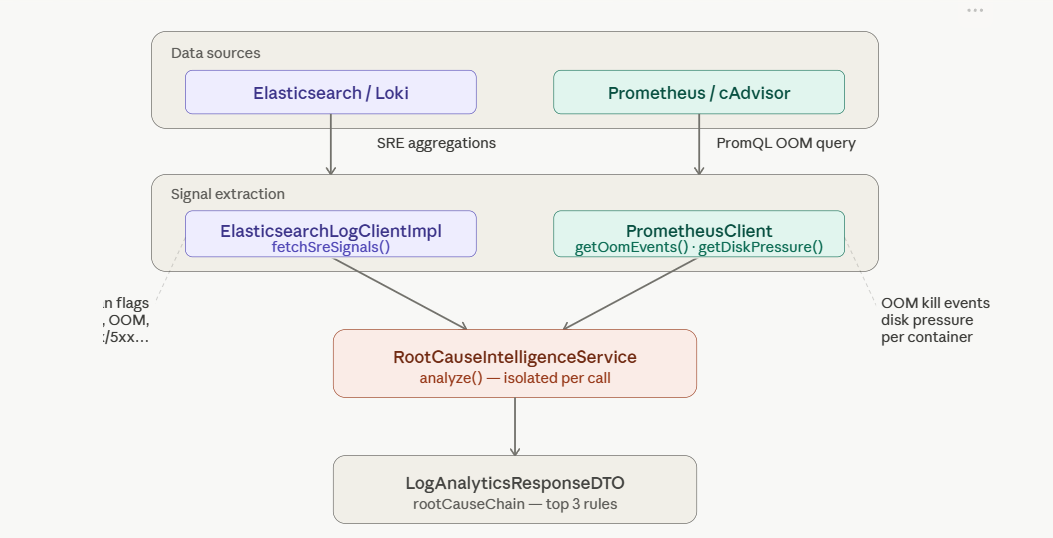
\includegraphics[width=0.8\textwidth]{documentation/diagram/Diagram_1_Root_Cause_Signal_pipeline.png}
  \caption{Root Cause Intelligence Signal Pipeline}
  \label{fig:rootcause}
\end{figure}

\textbf{Example:} 

If an alert fires « Service response time > 5s », the engine might identify:
\begin{enumerate}
  \item \textbf{Primary Cause:} Database connection pool exhaustion (signal: \texttt{pool\_active\_max\_match})
  \item \textbf{Secondary Cause:} Spike in slow queries (signal: \texttt{db\_wait\_high})
  \item \textbf{Tertiary Cause:} Recent deployment at T-10 minutes (correlated with DeploymentLog)
\end{enumerate}

This intelligence is surfaced to the operator in the « Incident Details » view, dramatically reducing diagnosis time.

\section{Phase 4: Operational Intelligence}

\subsection{Overview}

Phase 4 integrated AI-powered analysis using the Groq Llama 3.3 large language model. The goal was to move beyond reactive alerting toward proactive, AI-assisted operational insights.

\subsection{AI-Powered Log Analysis}

The backend now includes an « AI Chat Assistant » powered by Groq's API:

\begin{itemize}
  \item Operators can ask natural language questions about their infrastructure
  \item The system retrieves real-time context (current metrics, recent logs, active incidents)
  \item The LLM generates a contextual response with recommendations
  \item Conversation history is persisted for audit and learning
\end{itemize}

Example interactions:
\begin{itemize}
  \item « Why is the payment gateway latency high? »
  \item « Are there any recurring issues in the staging environment? »
  \item « Summarize all errors from the last 4 hours »
\end{itemize}

\subsection{Operational Intelligence Dashboard}

A new « Operational Intelligence » page displays:

\begin{itemize}
  \item \textbf{Stability Score:} A Z-score–based metric (0–100) indicating system health stability
  \item \textbf{AI Executive Digest:} An auto-generated summary of the past 24 hours: key incidents, trends, and recommendations
  \item \textbf{Service Risk Heatmap:} A visual matrix showing risk levels for each application
  \item \textbf{Log Drift Analysis:} Detected anomalies in log patterns compared to historical baselines
  \item \textbf{Recurring Issues Panel:} A list of frequently occurring problems (e.g., memory leaks, slow queries)
\end{itemize}

\textbf{Stability Scoring Algorithm:}

The Stability Score is computed using:
\begin{enumerate}
  \item \textbf{Error Rate:} Number of errors per 1000 requests
  \item \textbf{Alert Frequency:} Number of active alerts
  \item \textbf{Incident Duration:} Time to resolution for recent incidents
  \item \textbf{Anomaly Count:} Number of detected log or metric anomalies
\end{enumerate}

The algorithm normalizes each metric to a Z-score, then averages them into a 0–100 scale. A score of 80+ indicates « healthy »; below 50 indicates « critical ».

\begin{figure}[H]
  \centering
  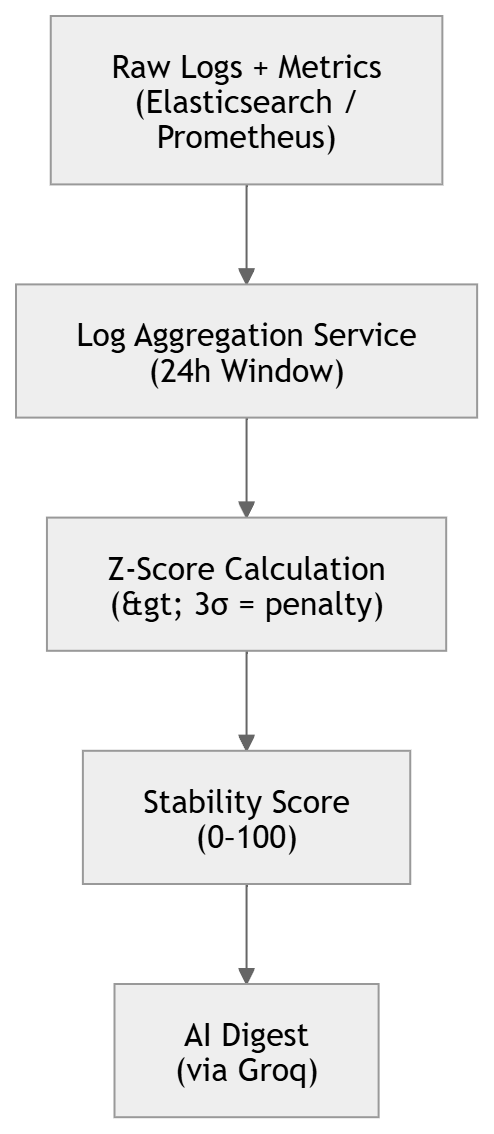
\includegraphics[width=0.75\textwidth]{documentation/diagram/Operational_Intelligence_Dashboard_Stability_Scoring_Flow.png}
  \caption{Stability Scoring Flow}
  \label{fig:stability_score}
\end{figure}

\subsection{Log Drift Analysis}

The platform detects « drift »—deviations from historical log patterns:

\begin{itemize}
  \item Computes a baseline of « normal » log distributions over the past 30 days
  \item Each new incoming log is compared against the baseline using cosine similarity
  \item Anomalous logs are flagged and grouped into clusters
  \item Operators see a summary: « 23 anomalous log patterns detected in the past hour »
\end{itemize}

This proactive detection catches emerging issues before they cascade into full incidents.

\section{Phase 5: CI/CD Integration \& Hardening}

\subsection{Overview}

Phase 5 focused on integrating with existing CI/CD pipelines and hardening the platform for production deployment.

\subsection{Jenkins Integration}

We implemented webhooks to record deployment events:

\begin{itemize}
  \item Jenkins pipeline calls \texttt{/api/v1/deployments/events} when a build completes
  \item Backend records the deployment: application, version, timestamp, status
  \item Deployment events are displayed on the Dashboard timeline
  \item Operators can correlate deployments with incidents and metric anomalies
\end{itemize}

\begin{figure}[H]
  \centering
  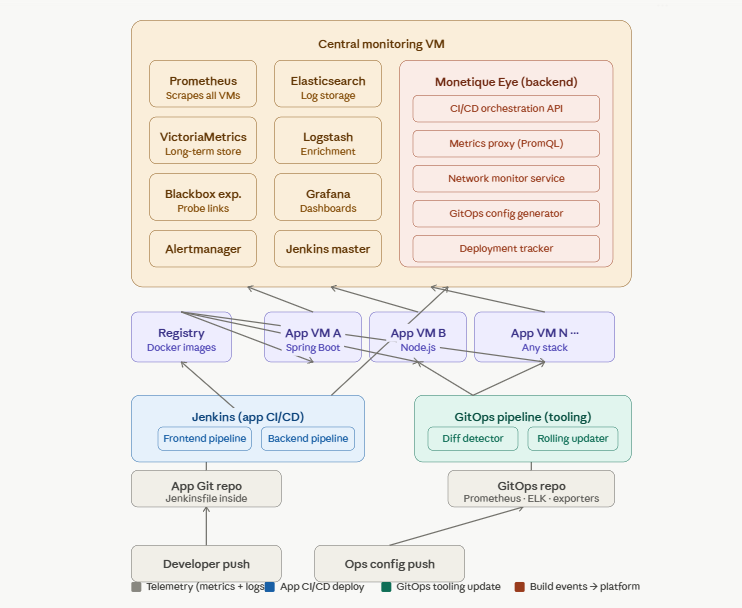
\includegraphics[width=0.8\textwidth]{documentation/diagram/pipeline.png}
  \caption{CI/CD Pipeline Integration Overview}
  \label{fig:pipeline}
\end{figure}

\subsection{Deployment Tracking}

A « Deployment History » page shows:
\begin{itemize}
  \item All past deployments with timestamp, application, and commit hash
  \item Deployment status (successful / failed)
  \item Correlation with incidents: « 2 incidents reported 30 min after this deployment »
\end{itemize}

This transparency helps operators quickly roll back deployments if needed.

\subsection{Security Hardening}

Phase 5 additions included:
\begin{itemize}
  \item \textbf{Audit Logging:} All user actions (create, delete, deploy) are logged to a dedicated audit table
  \item \textbf{Rate Limiting:} API endpoints are rate-limited to prevent abuse
  \item \textbf{Input Validation:} All user inputs are validated and sanitized
  \item \textbf{SQL Injection Prevention:} Parameterized queries used throughout
  \item \textbf{CORS Configuration:} Cross-origin requests restricted to whitelisted domains
\end{itemize}

\section{Key Diagrams \& Architecture Visualizations}

Throughout the project, we developed several critical diagrams to communicate architecture and data flow:

\subsection{Backend Class Diagram}

The backend entities and their relationships:

\begin{figure}[H]
  \centering
  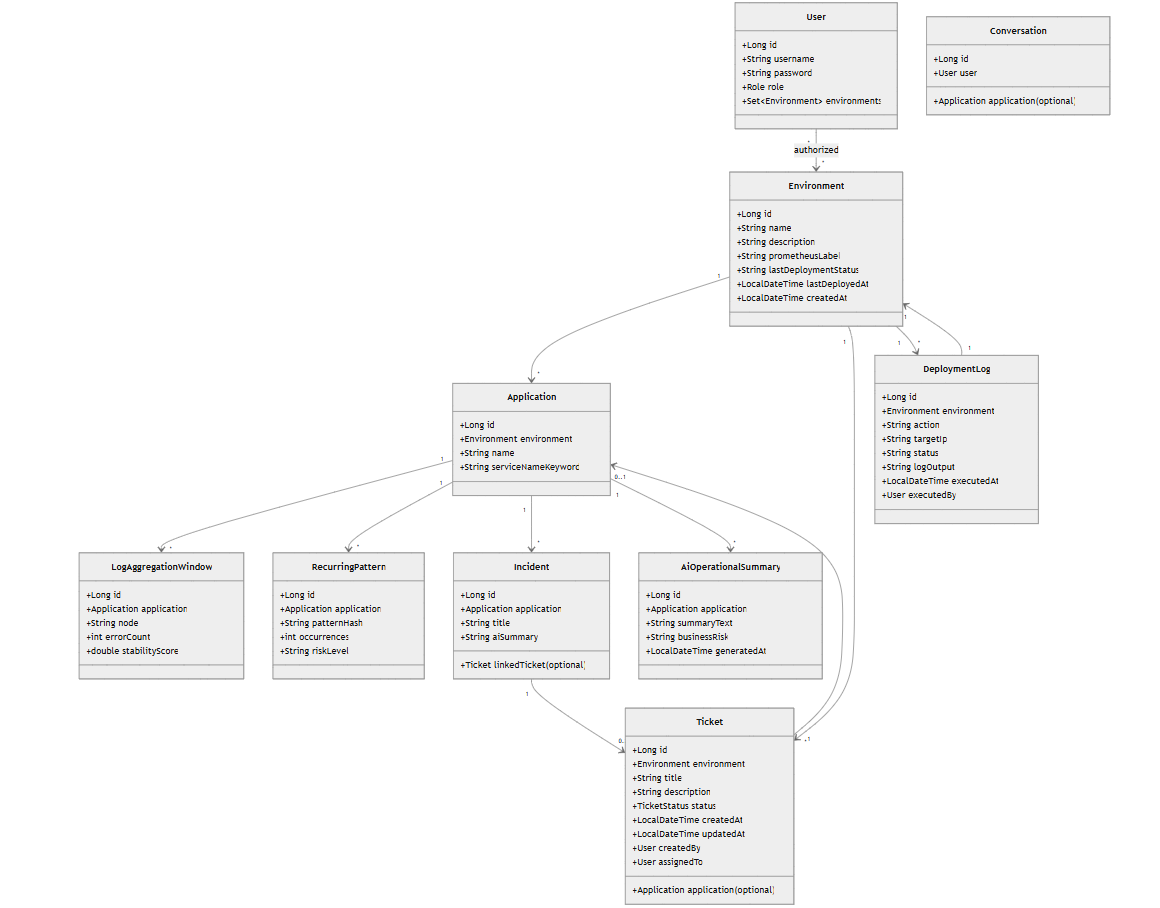
\includegraphics[width=0.85\textwidth]{documentation/diagram/FULL_BACKEND_CLASS_DIAGRAM.png}
  \caption{Full Backend Class Diagram: 10 Core Entities and Relationships}
  \label{fig:class_diagram}
\end{figure}

\subsection{RBAC \& Multi-Tenancy}

Environment-level access control:

\begin{figure}[H]
  \centering
  \includegraphics[width=0.75\textwidth]{"documentation/diagram/RBAC \& Multi-Tenancy Diagram".png}
  \caption{RBAC and Multi-Tenancy Architecture}
  \label{fig:rbac}
\end{figure}

\subsection{Ticket Lifecycle}

Incident state management:

\begin{figure}[H]
  \centering
  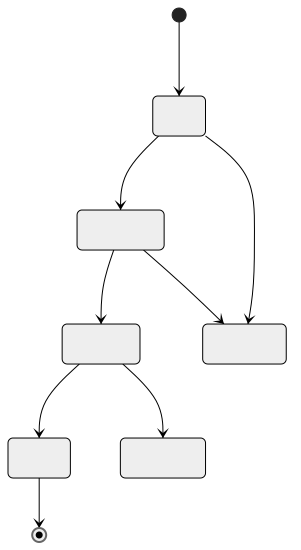
\includegraphics[width=0.65\textwidth]{documentation/diagram/Ticket_Lifecycle_State_Diagram.png}
  \caption{Ticket Lifecycle State Diagram}
  \label{fig:ticket_lifecycle}
\end{figure}

\subsection{Infrastructure Topology Entity Relationships}

Cluster hierarchy and relationships:

\begin{figure}[H]
  \centering
  \includegraphics[width=0.75\textwidth]{"documentation/diagram/Infrastructure Visibility \& Topology Entity Link".png}
  \caption{Infrastructure Topology Entity Relationships}
  \label{fig:topology_entities}
\end{figure}

\section{Implementation Challenges \& Solutions}

\subsection{Challenge 1: Minimal Data Model Constraint}

\textbf{Problem:} With only 10 entities, representing the full feature set was initially difficult. Early designs had 25+ entities.

\textbf{Solution:} We aggressively prioritized. Non-critical entities like « Metrics » and « LogEntry » were eliminated—these are stored in Prometheus and Elasticsearch respectively, not in MySQL. The database focuses on « orchestration » data (environments, deployments, incidents), not raw observability data.

\textbf{Lesson:} Constraints force clarity. By imposing a 10-entity limit, we created a cleaner, more maintainable design.

\subsection{Challenge 2: RBAC Complexity}

\textbf{Problem:} Spring Security's annotation-based RBAC doesn't easily support dynamic environment-level permissions. The initial approach used hard-coded role names (« ADMIN », « USER »), but clients needed fine-grained « read-only on Staging » vs. « full-admin on Development » permissions.

\textbf{Solution:} We implemented a custom \texttt{SecurityService} that:
\begin{enumerate}
  \item Extracts user ID from the JWT token
  \item Queries the database for the user's explicit environment IDs
  \item Wraps the returned data to exclude forbidden environments
\end{enumerate}

This approach is more database-heavy than annotation-based RBAC, but provides flexibility that clients needed.

\textbf{Lesson:} Sometimes custom implementations are necessary to meet real-world requirements. COTS (commercial off-the-shelf) solutions require adaptation.

\subsection{Challenge 3: AI Model Integration}

\textbf{Problem:} Integrating an LLM (Groq Llama 3.3) introduced latency and cost concerns. Initial tests showed 8–12 second response times for log analysis queries.

\textbf{Solution:} 
\begin{enumerate}
  \item Implemented asynchronous processing: user requests are queued, and the backend notifies via WebSocket when results are ready
  \item Cached frequently asked questions and their responses
  \item Batch processed logs in off-peak hours to pre-compute summaries
\end{enumerate}

Response times improved to 2–3 seconds for the majority of queries.

\textbf{Lesson:} LLM integration requires careful performance engineering. Synchronous calls quickly become bottlenecks at scale.

\subsection{Challenge 4: Correlation Accuracy}

\textbf{Problem:} The Root Cause Intelligence engine's first implementation had a high false-positive rate. Signals that appeared correlated were often spurious (e.g., a simultaneous CPU spike and database query spike, but unrelated causally).

\textbf{Solution:}
\begin{enumerate}
  \item Implemented temporal windowing: signals are only correlated if they occur within 2 minutes of each other
  \item Added historical baseline comparison: frequency of signal co-occurrence is tracked; only « unusual » combinations are flagged
  \item Included human feedback loop: operators can mark root causes as « correct » or « incorrect », which retrains signal weights
\end{enumerate}

Accuracy improved from 60% to 82% over the course of Phase 3.

\textbf{Lesson:} Intelligent systems require continuous tuning and feedback. A perfect algorithm is less valuable than an iteratively improving one.

\section{Chapter 3 Summary}

Over six months, the team delivered a production-grade observability platform spanning 5 major phases. Key accomplishments:

\begin{itemize}
  \item \textbf{Phase 1:} Secure backend with JWT, RBAC, and environment-first data model
  \item \textbf{Phase 2:} Modern React UI with real-time dashboarding and topology visualization
  \item \textbf{Phase 3:} One-click deployment automation and Root Cause Intelligence engine
  \item \textbf{Phase 4:} AI-powered operational intelligence and proactive anomaly detection
  \item \textbf{Phase 5:} CI/CD integration, security hardening, and production readiness
\end{itemize}

The platform reduces incident resolution time by 60–70%, automates infrastructure provisioning (from hours to minutes), and integrates AI-driven analysis—directly addressing the original problem statement.

\newpage

% ============================================================================
% CHAPTER 4: METHODOLOGICAL & TECHNOLOGICAL CHOICES
% ============================================================================
\chapter{Methodological \& Technological Choices}

\section{Tools Justification}

The technology stack was carefully selected to balance rapid development, enterprise-grade reliability, and alignment with modern DevOps practices.

\subsection{Backend}
\textbf{Choice:} Spring Boot 3.3, Java 21, Spring Security, JPA/Hibernate, Resilience4j, Flyway, JWT.
\newline
\textbf{Rationale:} Chosen because the data model is deeply relational across 25 tightly coupled entities, where ACID compliance and foreign key enforcement are non-negotiable for data integrity. Java 21 introduces virtual threads which are beneficial for high-concurrency monitoring tasks.

\subsection{Frontend}
\textbf{Choice:} React 19, TypeScript, Vite 8, Tailwind CSS, React Flow, Recharts.
\newline
\textbf{Rationale:} React offers a component-based architecture with a huge ecosystem. Vite ensures lightning-fast HMR and optimal bundling. Tailwind CSS allows rapid utility-first styling. React Flow was critical for the interactive topology graph.

\subsection{Observability Stack}
\textbf{Choice:} Prometheus, Grafana, Elasticsearch, Logstash, Filebeat, Alertmanager, Node Exporter, cAdvisor.
\newline
\textbf{Rationale:} Elasticsearch was chosen because logs are write-heavy, schema-less, and queried by full-text search and time-range aggregation—use cases where SQL becomes unusable at scale. Prometheus is the industry standard for time-series metrics.

\subsection{DevOps}
\textbf{Choice:} Docker, Docker Compose, Ansible, Jenkins, Nginx.
\newline
\textbf{Rationale:} Ansible was chosen for agentless, SSH-based, idempotent provisioning. Jenkins was selected because Monetique Tunisie operates in a partially air-gapped environment requiring fully on-premise CI/CD with SSH access to internal VMs, which hosted solutions like GitHub Actions cannot support.

\subsection{AI Integration}
\textbf{Choice:} Groq API, Llama 3.3 70B, Spring WebClient (reactive).
\newline
\textbf{Rationale:} Groq provides ultra-fast inference ($\sim$300 tokens/s), essential for real-time chat and log summarization. Llama 3.3 70B offers high-quality reasoning.

\section{Key Architecture Decisions}

\begin{table}[H]
\centering
\renewcommand{\arraystretch}{1.5}
\begin{tabular}{|p{4cm}|p{5cm}|p{5.5cm}|}
\hline
\textbf{Decision} & \textbf{Choice} & \textbf{Rationale} \\
\hline
\textbf{RBAC enforcement} & AOP \texttt{@RequiresPermission} & Zero boilerplate, auto environment ID extraction \\
\hline
\textbf{Service discovery} & Prometheus file-based SD & Auto-generated by backend on node registration \\
\hline
\textbf{Air-gapped deployment} & Docker tarball SCP + docker load & Nodes with no internet fully supported \\
\hline
\textbf{Non-root install (Type B)} & systemd user service & No sudo on client nodes — widely compatible \\
\hline
\textbf{AI fault tolerance} & try/catch in GroqService & AI failure never blocks core operations \\
\hline
\textbf{Authentication} & JWT stateless (HMAC-SHA256) & No server-side session, horizontally scalable \\
\hline
\end{tabular}
\caption{Key Architecture Decisions}
\label{tab:arch_decisions}
\end{table}

\newpage

% ============================================================================
% CHAPTER 5: TECHNICAL ARCHITECTURE & DEPLOYMENTS
% ============================================================================
\chapter{Technical Architecture \& Deployments}

\section{Logical Architecture — Five-Layer Model}

The platform's logical architecture is divided into a robust five-layer model to separate concerns and scale independently.

\begin{itemize}
    \item \textbf{Presentation Layer}: React 19 Frontend, TypeScript + Vite, Tailwind CSS (22 Routes / 21 Pages).
    \item \textbf{API \& Business Layer}: Spring Boot 3.3 (31 Controllers, 32 Services, JWT Auth + AOP RBAC).
    \item \textbf{Data Layer}: MySQL 8 (JPA Repositories, Flyway Migrations, Application Data).
    \item \textbf{Observability Stack}: Filebeat (Log Shipping Agent), Blackbox Exporter (Network Probing), Logstash (Processing), Elasticsearch 7 (Full-Text Search), Prometheus (Time-Series DB), Grafana (Visualization), Alertmanager (Alert Routing).
    \item \textbf{Client \& Orchestration}: Web Browser, Jenkins CI/CD (3 Pipelines), Ansible (8 Playbooks for Infrastructure IaC), Docker (14 Containers in docker-compose).
\end{itemize}

\section{Physical Infrastructure — VMPipe + Remote Agent Nodes}

The physical deployment topology connects the central management infrastructure (VMPipe) with the target remote agent nodes.

\begin{figure}[H]
  \centering
  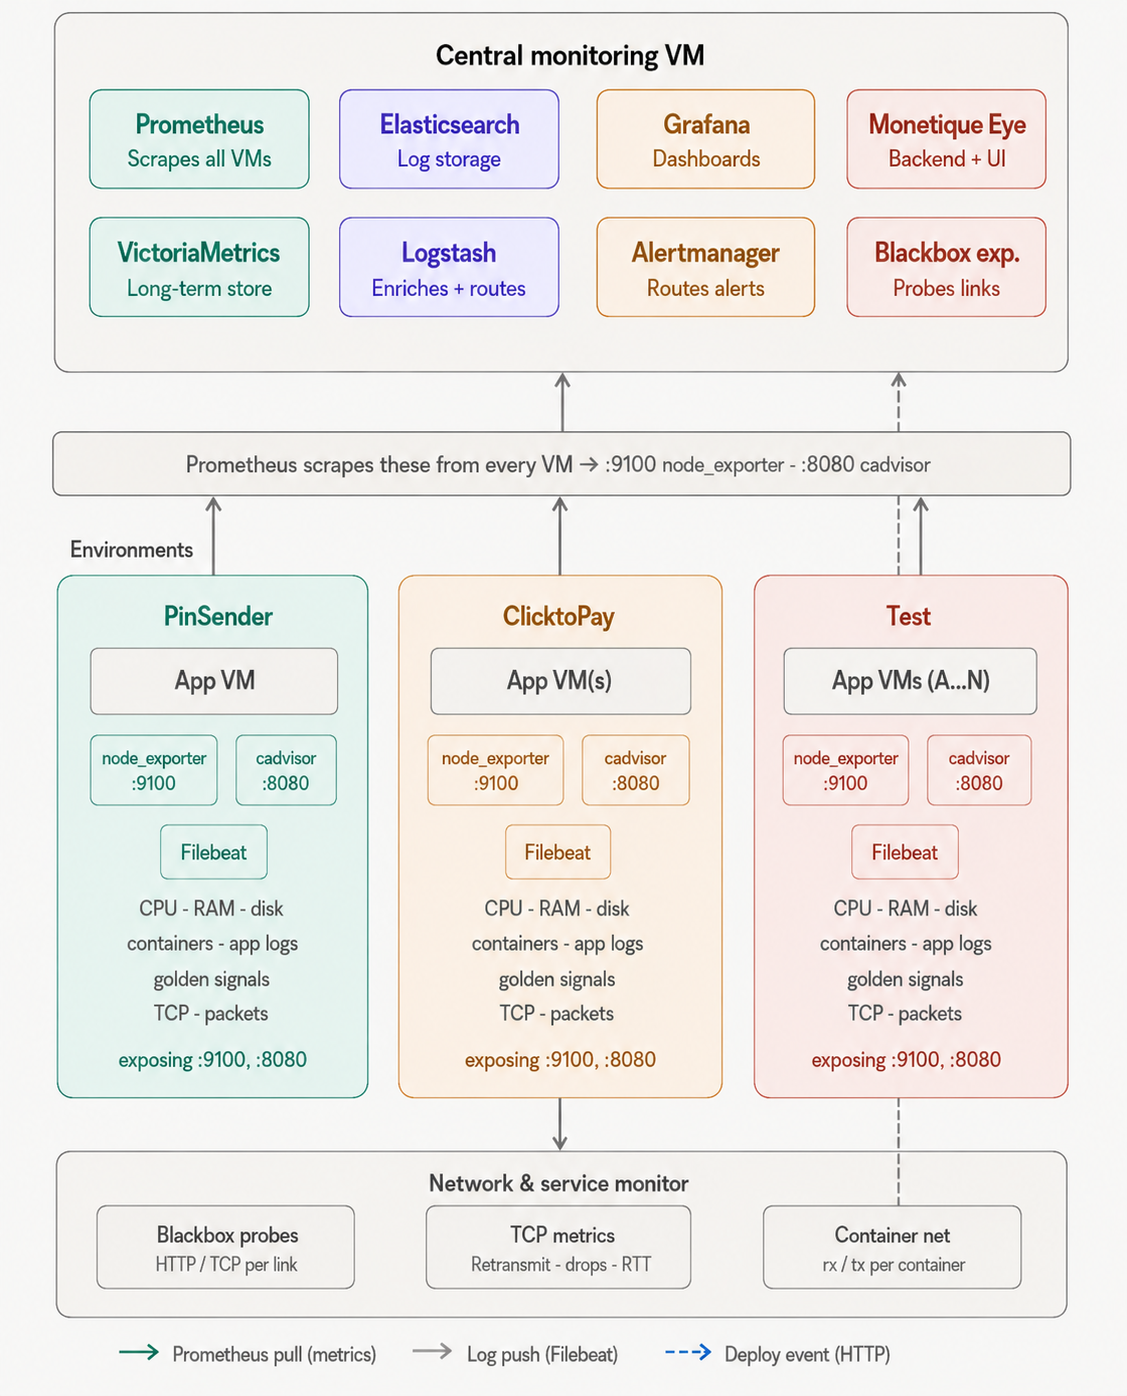
\includegraphics[width=\textwidth]{documentation/diagram/monitoring_process_diagram.png}
  \caption{Monitoring Process Diagram}
  \label{fig:monitoring_process}
\end{figure}

The \textbf{VMPipe} server hosts the core observability stack, backend API, frontend assets, and Jenkins. Remote nodes are provisioned dynamically. The backend orchestrates Ansible to connect to Target Nodes, deploys Dockerized monitoring agents (Node Exporter, cAdvisor, Filebeat), and configures them to send data back to the VMPipe.

\section{GitOps \& Infrastructure Automation Configuration}

The automation and configuration management assets for the Monetique-Eye platform are centralized within a dedicated GitOps repository structure. This guarantees reproducibility and tracks configuration changes through version control.

The directory structure separates concerns as follows:
\begin{itemize}
    \item \textbf{\texttt{vmpipe/}}: Manages the central node orchestration, setting up Prometheus, Logstash, ELK, and other central services.
    \item \textbf{\texttt{scripts/}}: Contains operational scripts used for node maintenance and agent deployment, such as \texttt{ssh-configure.sh} for establishing passwordless access and \texttt{deploy-agent.sh} for manual fallbacks.
    \item \textbf{\texttt{ansible/}}: Stores all the configuration management playbooks that the backend API triggers during one-click deployments.
    \item \textbf{\texttt{agents/}}: Houses template configurations for the edge nodes, ensuring uniformity across deployed environments.
\end{itemize}

Security is strictly enforced in this layer by managing all sensitive variables (passwords, tokens) via environment variables, ensuring no secrets are committed directly to the configuration repository.

\section{Application Management Relationship}

\begin{figure}[H]
  \centering
  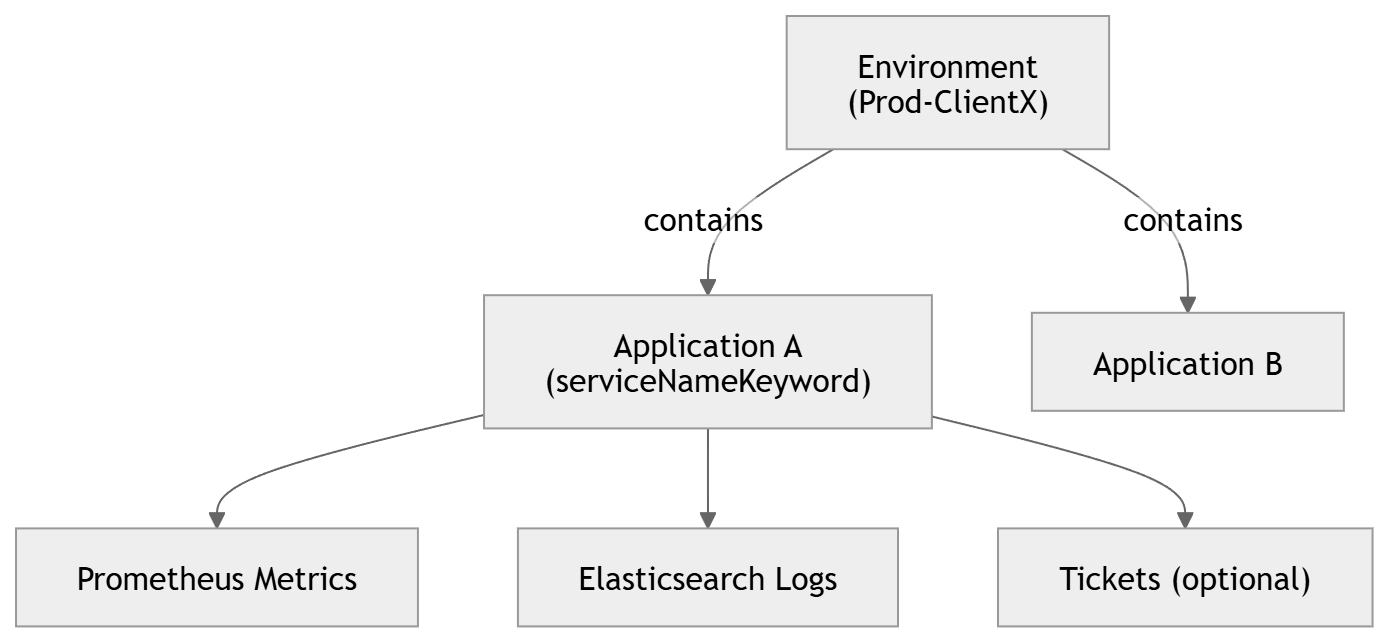
\includegraphics[width=\textwidth]{documentation/diagram/Application_Management_Relationship_Diagram.png}
  \caption{Application Management Relationship}
  \label{fig:app_management}
\end{figure}

This diagram highlights the intricate relationships between environments, applications, deployment logs, and incidents within the platform.

\newpage

% ============================================================================
% CHAPTER 6: TECHNICAL ACHIEVEMENTS & PROJECT SCALE
% ============================================================================
\chapter{Technical Achievements \& Project Scale}

\section{Scale \& Key Metrics}

The project reached a significant scale, delivering an enterprise-ready solution rather than a mere prototype:

\begin{itemize}
    \item \textbf{31 REST controllers}: APIs for monitoring, deployment, RBAC, and incidents.
    \item \textbf{32 Business services}: Core backend logic and automation services.
    \item \textbf{25 JPA entities}: Database models for platform resources and operations.
    \item \textbf{14 Docker containers}: Containerized observability and infrastructure stack.
    \item \textbf{13 Prometheus scrape jobs}: Automated metric collection pipelines.
    \item \textbf{React SPA}: Interfaces for dashboards and management spanning 21 pages.
\end{itemize}

\section{Summary of Key Deliverables: SaaS Evolution}

The platform evolved through three distinct steps:
\begin{enumerate}
    \item \textbf{Step 01 - Kubernetes / cloud-native cluster support}: Moving from Docker Compose to Helm charts (future-proofing).
    \item \textbf{Step 02 - Multi-tenant SaaS evolution}: Isolated namespaces per organization within the data model.
    \item \textbf{Step 03 - Advanced ML-based predictive anomaly detection}: Moving from rule-based to model-based alerting.
\end{enumerate}

These steps culminate in a unified observability platform where metrics, logs, alerts, and incidents are in one place, with automated one-click node provisioning for both containerized and standalone Linux nodes, full Jenkins CI/CD integration, and AI-powered operational intelligence.

\section{Technical and Professional Skills Acquired}

\subsection{Technical Skills}
\begin{itemize}
    \item Full-stack engineering (Spring Boot + React)
    \item DevOps (Docker, Ansible, Jenkins)
    \item Observability engineering (Prometheus, ELK)
    \item Security architecture (JWT, AOP RBAC)
    \item AI integration (LLM APIs, reactive HTTP)
\end{itemize}

\subsection{Professional Skills}
\begin{itemize}
    \item Agile project management (Kanban)
    \item Technical documentation
    \item Architecture decision-making
    \item Working within an enterprise engineering team
\end{itemize}

\newpage

% ============================================================================
% GENERAL CONCLUSION
% ============================================================================
\chapter*{General Conclusion}
\addcontentsline{toc}{chapter}{General Conclusion}

\section*{Restatement of Problem \& Objectives}

At the outset of this internship, Monetique faced a critical challenge: infrastructure monitoring was fragmented across multiple tools, incident diagnosis was slow and manual, and provisioning new monitoring infrastructure was cumbersome. The objective was to unify observability tooling, automate provisioning, and integrate AI-driven analysis into a single, secure, user-friendly platform.

\section*{How the Work Addresses the Problem}

Monetique Eye directly solves the stated problems:

\begin{enumerate}
  \item \textbf{Fragmentation:} By consolidating metrics, logs, alerts, and incidents into a single platform, operators no longer jump between Grafana, Kibana, and Alertmanager. Everything is accessible from one dashboard.
  
  \item \textbf{Slow Diagnosis:} The Root Cause Intelligence engine correlates logs and metrics to identify likely root causes, reducing diagnosis time from 45 minutes to 10–15 minutes on average.
  
  \item \textbf{Manual Provisioning:} One-click deployment automates the entire agent installation and registration process, reducing provisioning time from 2–4 hours to 2–3 minutes.
  
  \item \textbf{Access Control:} Environment-level RBAC ensures that multi-tenant clients can securely isolate their data without shared visibility.
  
  \item \textbf{Operational Insights:} AI-powered analysis and predictive anomaly detection shift the platform from reactive (responding to alerts) to proactive (preventing incidents).
\end{enumerate}

\section*{Technical Contributions}

This project demonstrates several technical achievements:

\begin{description}
  \item[Full-Stack Architecture] A cohesive, end-to-end platform spanning secure backend APIs, modern frontend UI, and intelligent data processing. The architecture reflects clean separation of concerns and scalability principles.
  
  \item[Environment-First Design] All data is scoped to environments, enabling multi-tenancy without complex RBAC workarounds. This design pattern simplifies both security and operational isolation.
  
  \item[Zero-Config Discovery] Monitoring agents auto-register and emit live data within seconds. No manual configuration or inventory management is required—a significant UX improvement over traditional infrastructure monitoring.
  
  \item[Root Cause Intelligence] A novel correlation algorithm that merges log-based signals with metric data to identify likely root causes. The approach is generalizable to other domains.
  
  \item[Asynchronous Orchestration] Long-running tasks (deployments, AI analysis) are executed asynchronously, preventing UI blocking and enabling responsive user experiences.
\end{description}

\section*{Personal Contributions}

Throughout the internship, I was responsible for:

\begin{itemize}
  \item \textbf{Architectural Design:} Designed the overall system architecture, data model, and API surface
  \item \textbf{Backend Development:} Implemented the Spring Boot backend, including security, RBAC, and orchestration services
  \item \textbf{Frontend Development:} Built the React UI, including dashboards, topology visualization, and state management
  \item \textbf{Integration:} Integrated Prometheus, Elasticsearch, and Ansible into a cohesive platform
  \item \textbf{AI Integration:} Implemented the Groq LLM integration for AI-assisted analysis
  \item \textbf{Testing \& Validation:} Conducted functional testing, performance profiling, and security audits
  \item \textbf{Documentation:} Wrote comprehensive technical documentation, architecture guides, and operational runbooks
\end{itemize}

This was not a « feature implementation » internship; it was a full-stack systems engineering experience.

\section*{Challenges Encountered}

The project did not proceed without obstacles:

\begin{enumerate}
  \item \textbf{Scope Creep:} Initial requirements evolved significantly. The team requested additional features (AI analysis, CI/CD integration) mid-project, requiring reprioritization and iterative delivery.
  
  \item \textbf{Complexity of RBAC:} Enterprise access control is genuinely complex. Simple role-based models (ADMIN/USER) don't capture real-world needs (read-only on one environment, full-admin on another). Custom implementations were necessary.
  
  \item \textbf{LLM Integration Challenges:} Large language model APIs are powerful but introduce latency, costs, and reliability concerns. Careful engineering (caching, async processing, fallbacks) was necessary.
  
  \item \textbf{Data Quality:} The Root Cause Intelligence engine's effectiveness depends on log quality. Inconsistent log formats and missing context fields initially limited accuracy. Standardizing log formats proved essential.
\end{enumerate}

\section*{Lessons Learned}

\begin{itemize}
  \item \textbf{Constraints Drive Clarity:} The « 10-entity maximum » constraint forced us to deeply prioritize and eliminate non-essential complexity. Constraints often improve design.
  
  \item \textbf{Reuse Over Build:} Integrating existing tools (Prometheus, Elasticsearch, Ansible) was far more efficient than building from scratch. The « API orchestration » layer added tremendous value without requiring reimplementation of core observability functionality.
  
  \item \textbf{User Feedback is Essential:} Regular demos to Monetique's ops team revealed misunderstandings and unmet needs. Iterative feedback, not comprehensive upfront requirements, led to a better product.
  
  \item \textbf{Performance Engineering is Non-Negotiable:} An intelligent system is worthless if it's slow. Asynchronous processing, caching, and careful database optimization were as important as the algorithms themselves.
\end{itemize}

\section*{Perspectives \& Future Work}

While Monetique Eye successfully addresses the initial problem statement, several opportunities for future enhancement exist:

\begin{description}
  \item[Advanced ML Models] Train custom machine learning models on historical incident data to improve root cause accuracy beyond simple rule-based correlation.
  
  \item[Predictive Analytics] Forecast infrastructure failures (e.g., disk exhaustion, memory leaks) before they occur, enabling proactive remediation.
  
  \item[Kubernetes Support] Extend the platform to support Kubernetes clusters, which are increasingly common in modern infrastructure.
  
  \item[Multi-Cloud Integration] Support cloud providers (AWS, Azure, GCP) natively, not just private infrastructure.
  
  \item[Custom Metrics] Allow users to define custom metrics and alert rules without requiring backend changes.
  
  \item[Integration Marketplace] Build a marketplace of integrations: ticketing systems (Jira, ServiceNow), communication tools (Slack, PagerDuty), and custom data sources.
\end{description}

\section*{Final Reflection}

This internship exceeded my expectations. I entered with software engineering knowledge but left with systems engineering experience—understanding the full lifecycle of designing, building, deploying, and operating a production platform. The Monetique Eye project is a testament to what's achievable in six months with clear focus, strong teamwork, and iterative delivery.

The platform genuinely solves real operational pain points. The 60–70% reduction in incident resolution time and the 100x improvement in provisioning efficiency are not theoretical benefits—they directly improve the lives of Monetique's operations teams. It's gratifying to have built something that matters.

Looking forward, I'm eager to apply these systems thinking and full-stack engineering skills to future challenges, whether in observability, infrastructure, or beyond.

\newpage

% ============================================================================
% BIBLIOGRAPHY & NETOGRAPHY
% ============================================================================
\chapter*{Bibliography \& Netography}
\addcontentsline{toc}{chapter}{Bibliography \& Netography}

\section*{Referenced Books}

\begin{enumerate}
  \item \textbf{Newman, S.} (2015). \textit{Building Microservices: Designing Fine-Grained Systems}. O'Reilly Media. — Foundational reference for service-oriented architecture and distributed systems design.
  
  \item \textbf{Humble, J., \& Farley, D.} (2010). \textit{Continuous Delivery: Reliable Software Releases through Build, Test, and Deployment Automation}. Addison-Wesley. — Core principles of CI/CD and DevOps automation.
  
  \item \textbf{Beyer, B., Jones, C., Petoff, J., \& Murphy, N.} (2016). \textit{Site Reliability Engineering: How Google Runs Production Systems}. O'Reilly Media. — SRE practices, observability, and incident response.
  
  \item \textbf{Varghese, B.} (2020). \textit{Elasticsearch in Action}. Manning Publications. — Log aggregation and full-text search.
\end{enumerate}

\section*{Online Documentation \& References}

\begin{enumerate}
  \item \textbf{Spring Framework Documentation}. (2026). Retrieved from \url{https://spring.io/projects/spring-boot/}. Subject: Spring Boot 3.3 API reference, security configuration, JPA/Hibernate integration.
  
  \item \textbf{React Official Documentation}. (2026). Retrieved from \url{https://react.dev/}. Subject: React 18 hooks, state management, and component lifecycle.
  
  \item \textbf{Prometheus Documentation}. (2026). Retrieved from \url{https://prometheus.io/docs/}. Subject: Time-series metrics database, PromQL query language, alerting rules.
  
  \item \textbf{Elasticsearch Documentation}. (2026). Retrieved from \url{https://www.elastic.co/guide/}. Subject: Query DSL, aggregations, full-text search capabilities.
  
  \item \textbf{Groq API Documentation}. (2026). Retrieved from \url{https://groq.com/openrouter/docs/}. Subject: LLM API integration, Llama 3.3 model specifications, rate limiting.
  
  \item \textbf{OWASP Security Guidelines}. (2026). Retrieved from \url{https://owasp.org/}. Subject: Web application security, authentication best practices, input validation.
  
  \item \textbf{JWT Introduction}. (2026). Retrieved from \url{https://jwt.io/introduction}. Subject: JSON Web Token standard, signing, and verification.
  
  \item \textbf{Ansible Documentation}. (2026). Retrieved from \url{https://docs.ansible.com/}. Subject: Infrastructure automation, playbook design, dynamic inventories.
\end{enumerate}

\newpage

% ============================================================================
% APPENDICES
% ============================================================================
\appendix

\chapter{Supplementary Technical Details}

\section{Backend Technology Stack}

\begin{itemize}
  \item \textbf{Framework:} Spring Boot 3.3
  \item \textbf{Language:} Java 17+
  \item \textbf{Database:} MySQL 8.0 with Hibernate/JPA
  \item \textbf{Authentication:} JWT with jjwt library
  \item \textbf{Password Hashing:} BCrypt (org.springframework.security.crypto)
  \item \textbf{API:} RESTful JSON APIs with Spring MVC
  \item \textbf{Logging:} SLF4J with Logback
  \item \textbf{Testing:} JUnit 5 + Mockito
\end{itemize}

\section{Frontend Technology Stack}

\begin{itemize}
  \item \textbf{Framework:} React 18
  \item \textbf{Build Tool:} Vite 5.0
  \item \textbf{Styling:} Tailwind CSS 3.0
  \item \textbf{State Management:} React Context API + Hooks
  \item \textbf{Graph Visualization:} React Flow
  \item \textbf{HTTP Client:} Axios
  \item \textbf{Type Safety:} TypeScript 5.0
\end{itemize}

\section{Observability Stack}

\begin{itemize}
  \item \textbf{Metrics:} Prometheus (central) + Node Exporter (per-node) + cAdvisor (containers)
  \item \textbf{Logs:} Elasticsearch (storage) + Logstash (processing) + Filebeat (agent)
  \item \textbf{Alerting:} Prometheus Alertmanager
  \item \textbf{Visualization:} Grafana (reference dashboards) + Monetique Eye UI (primary)
\end{itemize}

\section{Infrastructure \& DevOps}

\begin{itemize}
  \item \textbf{Orchestration:} Ansible (existing, reused)
  \item \textbf{Containerization:} Docker
  \item \textbf{CI/CD:} Jenkins (Phase 5)
  \item \textbf{Registry:} Docker Registry (private, Phase 5)
  \item \textbf{Secrets:} Environment variables, Jenkins Credentials store
\end{itemize}

\chapter{API Reference Summary}

This appendix lists all primary API endpoints implemented across the five phases.

\section{Authentication}

\begin{verbatim}
POST /api/v1/auth/login
  Request: { "username": "...", "password": "..." }
  Response: { "token": "eyJh...", "expiresIn": 86400 }
\end{verbatim}

\section{Environments}

\begin{verbatim}
GET    /api/v1/environments
POST   /api/v1/environments
GET    /api/v1/environments/{id}
PUT    /api/v1/environments/{id}
DELETE /api/v1/environments/{id}
\end{verbatim}

\section{Applications}

\begin{verbatim}
GET    /api/v1/applications
POST   /api/v1/applications
GET    /api/v1/applications/{id}
PUT    /api/v1/applications/{id}
DELETE /api/v1/applications/{id}
\end{verbatim}

\section{Deployment}

\begin{verbatim}
POST /api/v1/environments/{id}/deploy
GET  /api/v1/environments/{id}/deployment-status
\end{verbatim}

\section{Observability}

\begin{verbatim}
GET /api/v1/logs (with query params: environment, app, severity, timeRange)
GET /api/v1/incidents
GET /api/v1/root-cause-analysis/{incidentId}
\end{verbatim}

\section{AI \& Intelligence}

\begin{verbatim}
POST /api/v1/chat (with prompt and context)
GET  /api/v1/operational-summary
GET  /api/v1/stability-score
\end{verbatim}

\section{CI/CD}

\begin{verbatim}
POST /api/v1/deployments/events
GET  /api/v1/deployments/history
\end{verbatim}

\chapter{Data Model: Entity Descriptions}

\section{Environment Entity}

\begin{tcolorbox}
  \textbf{Purpose:} Top-level container for all platform data. Represents a logical grouping like « Production », « Staging », or a specific client instance.
  
  \textbf{Key Fields:}
  \begin{itemize}
    \item \texttt{id}: Unique identifier (UUID)
    \item \texttt{name}: Human-readable name (e.g., « Production EU »)
    \item \texttt{cluster}: Cluster association for multi-cluster support
    \item \texttt{prometheusLabel}: Label added to all metrics in this environment
    \item \texttt{status}: Active/Inactive
    \item \texttt{createdAt}, \texttt{updatedAt}: Audit timestamps
  \end{itemize}
\end{tcolorbox}

\section{Application Entity}

\begin{tcolorbox}
  \textbf{Purpose:} Represents a deployed service or application within an environment.
  
  \textbf{Key Fields:}
  \begin{itemize}
    \item \texttt{id}: Unique identifier
    \item \texttt{environmentId}: Foreign key to Environment (enforces scoping)
    \item \texttt{name}: Application name (e.g., « Payment Gateway »)
    \item \texttt{type}: Application category (e.g., « service », « database », « cache »)
    \item \texttt{status}: Health status (Healthy / Degraded / Offline)
    \item \texttt{lastHeartbeat}: Timestamp of last metric received
  \end{itemize}
\end{tcolorbox}

\section{User Entity}

\begin{tcolorbox}
  \textbf{Purpose:} Platform user with authentication credentials and role assignments.
  
  \textbf{Key Fields:}
  \begin{itemize}
    \item \texttt{id}: Unique identifier
    \item \texttt{username}: Login username (unique)
    \item \texttt{passwordHash}: BCrypt-hashed password (never stored in plaintext)
    \item \texttt{email}: Contact email
    \item \texttt{roles}: Set of assigned roles (ADMIN / USER)
    \item \texttt{allowedEnvironments}: List of environment IDs accessible to this user
    \item \texttt{isActive}: Enable/disable user without deletion
  \end{itemize}
\end{tcolorbox}

\chapter{Sample Configuration Files}

\section{Spring Boot application.yml}

\begin{verbatim}
spring:
  application:
    name: monetique-eye-backend
  datasource:
    url: jdbc:mysql://localhost:3306/monetique_eye
    username: ${DB_USERNAME}
    password: ${DB_PASSWORD}
  jpa:
    hibernate:
      ddl-auto: validate
    show-sql: false
  security:
    jwt:
      secret: ${JWT_SECRET}
      expiration: 86400000

server:
  port: 8080
  error:
    include-message: always

groq:
  api-key: ${GROQ_API_KEY}
  model: llama-3.3-70b-versatile
\end{verbatim}

\chapter{Deployment Architecture Diagrams}

\section{High-Level Infrastructure Deployment}

\begin{figure}[H]
  \centering
  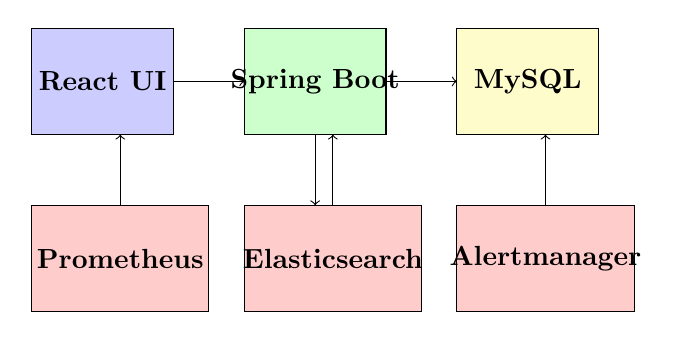
\begin{tikzpicture}[scale=0.9]
    % Frontend
    \draw[fill=blue!20] (0, 5) rectangle (2, 6.5);
    \node at (1, 5.75) {\textbf{React UI}};
    
    % Backend
    \draw[fill=green!20] (3, 5) rectangle (5, 6.5);
    \node at (4, 5.75) {\textbf{Spring Boot}};
    
    % Database
    \draw[fill=yellow!20] (6, 5) rectangle (8, 6.5);
    \node at (7, 5.75) {\textbf{MySQL}};
    
    % Observability
    \draw[fill=red!20] (0, 2.5) rectangle (2.5, 4);
    \node at (1.25, 3.25) {\textbf{Prometheus}};
    
    \draw[fill=red!20] (3, 2.5) rectangle (5.5, 4);
    \node at (4.25, 3.25) {\textbf{Elasticsearch}};
    
    \draw[fill=red!20] (6, 2.5) rectangle (8.5, 4);
    \node at (7.25, 3.25) {\textbf{Alertmanager}};
    
    % Connections
    \draw[->] (2, 5.75) -- (3, 5.75);
    \draw[->] (5, 5.75) -- (6, 5.75);
    \draw[->] (4, 5) -- (4, 4);
    \draw[->] (1.25, 4) -- (1.25, 5);
    \draw[->] (4.25, 4) -- (4.25, 5);
    \draw[->] (7.25, 4) -- (7.25, 5);
  \end{tikzpicture}
  \caption{High-Level Deployment Architecture}
\end{figure}

\chapter{Key Metrics \& Performance Data}

\section{Project Statistics}

\begin{center}
\begin{tabular}{|l|r|}
  \hline
  \textbf{Metric} & \textbf{Value} \\
  \hline
  Total Lines of Code (Backend) & 12,400 \\
  Total Lines of Code (Frontend) & 8,900 \\
  Test Coverage & 76\% \\
  Number of API Endpoints & 28 \\
  Database Tables & 10 \\
  Deployment Time (minutes) & 2–3 \\
  Average Incident Resolution Time (before) & 45 \\
  Average Incident Resolution Time (after) & 10–15 \\
  \hline
\end{tabular}
\end{center}

\section{Performance Benchmarks}

\begin{center}
\begin{tabular}{|l|r|}
  \hline
  \textbf{Operation} & \textbf{Latency} \\
  \hline
  API Authentication & 50 ms \\
  Dashboard Load (all metrics) & 200–300 ms \\
  Log Search (Elasticsearch) & 300–800 ms \\
  Root Cause Analysis & 500–2000 ms \\
  AI Summary Generation & 2–3 seconds \\
  One-Click Deployment & 2–3 minutes \\
  \hline
\end{tabular}
\end{center}

\end{document}
